\chapter{Etat de l'art sur les méthodes  }%40 références et 15 à 20 pages
\label{Etat_art_methode}
\minitoc
\newpage
\section{Introduction}
Dans ce chapitre, on propose un état de l'art sur deux outils particuliers que nous allons utilisés pour traiter le problème \textbf{SMEPC}.  Ces deux outils sont la programmation dynamique et l'apprentissage automatique. On présente aussi quelques généralités sur les techniques de modélisation par programmation linéaire.

\section{Généralités sur la modélisation}

\subsection{Généralités sur la programmation linéaire en nombres entiers}
%Faire 3 pages
Un programme mathématique est un problème d'optimisation sous contraintes, c'est à
dire qu'il consiste à minimiser (ou maximiser) une fonction sous contraintes. Un programme mathématique est un programme linéaire (PL) si la fonction-objectif
et les conditions à respecter sont linéaires. On parle de programme linéaire en
nombres entiers (PLNE) lorsque les valeurs des variables du programme linéaire doivent
être des nombres entiers alors qu'un programme linéaire mixte (PLM) est obtenu lorsque
certaines variables doivent être entières et d'autres pas.
Modéliser un problème de tournées de véhicules par un PL ou PLNE revient donc à
définir :
\begin{itemize}[label=$\square$]
	\item les variables de décision, représentant les décisions qui doivent être prises, par exemple le choix
	du véhicule qui visite chaque client, l'ordre de visite des clients, etc.
	\item  la fonction-objectif exprimée en fonction des variables, représentant le ou les objectifs
	à remplir, les termes à maximiser ou minimiser ;
	\item les contraintes exprimées en fonction des variables, représentant les conditions ou
	limites (capacité, logiques, temporelles, etc.) à prendre en compte lors de la construction de solutions réalisables. Les variables de décision et la fonction objectif à optimiser sont soumises aux contraintes . Il existe plusieurs types de contraintes : 
	\begin{itemize}
		\item les contraintes d'intégrités ou de signe;
		\item les contraintes d'inégalité par exemple $Ax \leq b $;
		\item les contraintes d'égalité par exemple $Ax = b $.
	\end{itemize}
\end{itemize}
On donne une définition plus formelle d'un PLNE à la définition (\ref{PLNED}).
Relaxer un PLNE ou un PLM consiste en général à supprimer certaines de ses contraintes,
ou alors les remplacer par des contraintes plus faibles. Le problème résultant est souvent
plus simple à résoudre que l'original, mais si la relaxation est bien faite alors sa solution
optimale peut être réalisable pour le problème original, et donc optimale pour ce dernier,
ou alors ne pas être réalisable mais avoir un coût proche de l'optimum du problème original. On donne une définition plus formelle de la relaxation d'un PLNE à la définition (\ref{RPLNED}).

\begin{Def} 
	\label{PLNED}\cite{Sakar84}
	soient $A$ une matrice de taille $n \times m$, $b$ un vecteur colonne de taille $m$ et $c$ un vecteur ligne de taille $n$. Un programme linéaire en nombres entiers est le problème d'optimisation suivant : 
	
	$$
	(P) \left\{
	\begin{array}{ll}
	Ax \leq b   \\
	z=Max(cx) \textrm{ ou } Min(cx)\\ 
	\end{array}
	\right.
	$$
	
	avec $x=(x_j \in \pmb{\mathbb{N}}$, $j = \{1, 2, \dots, n\})$,  $x$ est un vecteur  inconnu de taille $n$ et la fonction objectif $z$ est une fonction linéaire à maximiser ou à minimiser. On dit qu'on a un programme linéaire en variables bivalentes si les contraintes $x_j \in \pmb{\mathbb{N}}$ sont remplacées par $x_j \in \{0,1\}$.
\end{Def}


\begin{Def}\cite{Sakar84}
	\label{RPLNED}
	Quand on relâche les contraintes d'intégrité sur les variables ($x_j \in \pmb{\mathbb{N}}$) dans le programme linéaire en nombres entiers $P$ de la définition \ref{PLNED}, on obtient le programme linéaire suivant : 
	
	$$
	(P') \left\{
	\begin{array}{ll}
	Ax \leq b   \\
	z=Max(cx) \textrm{ ou } Min(cx)\\ 
	\end{array}
	\right.
	$$
	
	avec $x_j \geq 0$, $j = \{1,2,...,n\}$ . 
\end{Def}

Il existe une relation entre $P$ et  $P'$ : si par hasard, la solution optimale de $P'$ est entière, c'est aussi une solution de $P$.

Généralement, les méthodes exactes permettent de trouver des solutions optimales en temps polynomial pour des problèmes de petite taille. Mais lorsque les problèmes sont de grande taille ces techniques ont du mal à  trouver des solutions. Pour pouvoir traiter des problèmes de plus grande taille, on peut enrichir nos programmes avec certaines techniques comme par exemple le \textit{Branch-And-Cut (B\&C)}.


\subsection{Généralités sur la technique de \textit{Branch-And-Cut (B\&C)}}
La génération de coupes est une méthode utilisée quand le programme linéaire possède un très grand nombre de contraintes (par exemple exponentiel par rapport au nombre de variables). 
Soit $P$ un programme linéaire (aussi appelé modèle dans la terminologie Cplex) et $C$ l'ensemble des contraintes de $P$. L'idée est d'essayer de résoudre le modèle $P$ sans être obligé d'y inclure explicitement toutes les contraintes. On forme alors le modèle initial $P_0$ avec un sous-ensemble $C_0 \subset C$ des contraintes, on le résout et on examine la solution. Si la solution est valide (i.e. toutes les contraintes de $C$ sont respectées) alors on a la solution optimale. Sinon on ajoute au modèle les contraintes dans $C$ violées par la solution. On recommence itérativement ce processus jusqu'à obtenir une solution qui respecte toutes les contraintes. On espère atteindre cette solution avant d'avoir intégré explicitement toutes les contraintes au modèle.
Remarquons qu'on appelle coupes les contraintes ajoutées itérativement au modèle car elles coupent (i.e. rendent invalide) la solution courante.

\section{Programmation dynamique}

%La \textit{Programmation Dynamique} (PD) a été initialement proposée par  en 1987 en reprenant le principe de la méthode de relaxation mise au point par \cite{ChrMinTot81tsptw} pour le VRP. 
La \textit{Programmation Dynamique} (PD) \cite{doi:10.1126/science.153.3731.34} \cite{brown1965iterative} \cite{karp1967finite} \cite{mitten1964composition} \cite{nemhauser1966introduction}  %\ref{denardo1966m}
 constitue un outil, à la fois outil algorithmique et de modélisation, destiné à la gestion de \textit{trajectoires}, c'est-à-dire de séquences de transitions d'un système qui obéit à une logique physique ou économique propre, mais sur lequel un acteur humain est supposé agir. Un point essentiel pour que la recherche de telles trajectoires soit justifiable est que leurs performances s'expriment comme une \textit{somme} (application d'un opérateur associatif) de performances de leurs transitions. Dès lors, d'un point de vue algorithmique, les processus de programmation dynamique peuvent souvent être vus comme des processus de recherche de chemins dans un graphe sans circuit, ou le cas échéant de circuits quand les trajectoires sont cycliques, et font souvent dès lors référence au principe dit de Bellman. Dans le cas où le temps est continu, on parle souvent de \textit{Contrôle Optimal}, et le principe de Bellman se décline alors sous forme d'équations différentielles. 

Les applications sont multiples : Gestion de production et gestion de stock en contexte industriel,  contrôle de trajectoire en aéronautique,  gestion de portefeuille (contrôle optimal stochastique) en Finance de Marché, procédés dits du \textit{Split} en Algorithmique de l'Optimisation de Tournées. 
\subsection{Cadre général}
\label{Cadre_general}
Afin de rendre plus lisible la présentation de ce cadre général, on va s'appuyer ici sur un exemple simple :
\begin{enumerate}
	\item	On considère une usine $U$ qui produit chaque jour des quantités d'un produit unique $P$. Chaque soir, cette usine livre le contenu de sa commande au(x) client(s) : on travaille ici sur un ensemble de 30 jours, numérotés $i = 1,\dots, 30 = N$, et la quantité à livrer chaque soir est connue et de valeur $L_i$ ;
	\item	L'usine est contrainte par des contraintes de capacité :
	\begin{itemize}[label=$\square$]
		\item	Capacité de stockage de la production d'un jour à l'autre : à un instant donné, l'usine de stockage ne peut accueillir plus de $C^{Stock}$ unités de produit ;
		\item	Capacité de production : sur une journée, $U$ ne peut produire plus de $C^{Prod}$ unités de produit. Ce rendement peut toutefois être augmenté jusqu'à un niveau $C^{Prod\_Sup} > C^{Prod}$ dès lors que l'usine loue une certaine machine $M$.
		
	\end{itemize}
	\item	L'usine a enfin à s'acquitter de coûts : 
	\begin{itemize}[label=$\square$]
		\item	Coût de stockage : Si la quantité $\alpha$ de produit stockée est non nulle alors stocker $\alpha$ unités de produit pendant une nuit à un coût $Fix\_Stock + \alpha \times Var\_Stock$, sinon ce coût de stockage est nul. 
		\item	Coût de production : Si la quantité $\beta$ de produit réalisée au jour $i$ est non nulle alors produire $\beta$ unités de produit au jour $i$ a un coût $Fix\_Prod_i + \beta \times Var\_Prod_i$, sinon ce coût de production est nul.
		\item	Coût de location/installation de machine, qui traduit le fait qu'utiliser la machine $M$ a un coût : 
		\begin{itemize}
			\item	Coût d'installation $Install_i$, si l'installation est réalisée durant la nuit qui conclut le jour i ; On considère que si $M$ est utilisée deux (ou plus) jours consécutifs, elle n'a pas à être enlevée et donc elle n'est installée qu'une fois. Par contre, si elle cesse à un jour donné d'être utilisée (louée) alors elle doit être désinstallée et rendue (la désinstallation s'effectue le soir après utilisation, ce qui fait que si elle est à nouveau utilisée un peu plus tard, elle doit être à nouveau installée.
			\item Coût de location par jour d'utilisation : $Loc_i$.
			
		\end{itemize}
		\item 	La fonction à optimiser est une fonction séparable. Compte tenu de tout cela, on veut donc produire et stocker de façon à satisfaire la demande (contraintes) tout en minimisant le coût (performance). 
	\end{itemize}
\end{enumerate}
Cet exemple va nous permettre d'illustrer ce que sont les principaux composants d'un modèle (et aussi d'un algorithme) de \textit{Programmation Dynamique}. Ceux-ci sont les suivants : 
\begin{itemize}[label=$\square$]
	\item Un Espace-Temps $\mathcal{T}$ ;
	\item Un Espace d'Etats  $E$ ;
	\item Un Espace de Décisions $D$ et de Transitions $TR$ Associées ;
	%\item Une mesure de Performance et Principe de Bellman ;
	%\item Un contexte d'Utilisation et 
	\item Une Stratégie d'Implémentation du Principe de Bellman;
	\item Les procédés de Filtrage.
\end{itemize}

\textbf{Un Espace-Temps $\mathcal{T}$} : Cet \textit{espace-temps} peut être \textbf{continu}, assimilé en général à l'espace $\mathbb{R}$  des nombres réels ou à un intervalle $[0, TMax]$. Il peut être aussi \textbf{discret}, muni d'un ordre partiel $<<$. Dans le cas où cet ordre est linéaire (Deux éléments sont toujours comparables), on pose souvent $\mathcal{T} = {0,\dots, N}$. Il peut enfin être \textbf{cyclique}, ce qui signifie que le processus que l'on cherche à optimiser a vocation à être périodique. Dans ce dernier cas on considère implicitement que N coïncide avec $0$ (ou $TMax$ avec $0$). 

\textbf{Dans le cas de notre exemple}, l'espace-temps sera bien entendu l'espace $\mathcal{T} = {0, 1, \dots, N, N+1}$ des jours, augmenté de deux jours fictifs $0$ et $N+1$ afin de pouvoir poser les bilans en début et fin de processus. Cet ensemble $\mathcal{T}$ est discret et ordonné de façon linéaire. Dans nos algorithmes, on utilisera la notation $i$ (au lieu de $t$) pour désigner un instant.

\textbf{Un Espace d'Etats E} : Un \textit{état} $e \in E$, associé à un instant $t \in \mathcal{T}$, est une description de l'état du système considéré à cet instant $t$. Il est généralement fourni au travers d'un ensemble de variables prenant des valeurs numériques (indicateurs de stock, température, vitesse, position, etc) ou booléennes (propriétés), voire des valeurs plus complexes telles que des listes, représentatives par exemple d'historiques.  De ce fait, une partie de la difficulté liée à la mise en œuvre de schémas DP tient au fait que ces états sont trop nombreux pour être énumérés, voire même infinis. 

Parmi ces états se trouve généralement un \textbf{Etat Initial} $e_0$, associé à l'instant initial $t = 0$, ainsi qu'une classe d'Etats Finaux, associé à l'instant $N$ ou $TMax$, et caractérisés par une propriété particulière. Ceci est bien entendu remis en cause quand l'horizon est cyclique.  

Il est important aussi de remarquer qu'à un instant donné $t$, tous les états de $E$ ne sont pas forcément possibles. Il est donc important de parvenir à filtrer, c'est-à-dire à identifier à chaque instant $t$, l'ensemble $E(t)$  des états possibles et pertinents.

\textbf{Dans le cas de notre exemple}, il faut pour définir notre espace d'états, s'entendre sur le moment précis où cet état est constaté : un état est en fait une photo instantanée du système, et, le système étant évolutif, il est essentiel d'être précis sur l'instant auquel cette photo est prise. On considèrera ici que l'état de notre usine est considéré au petit matin du jour $i$, avant qu'ait été lancée la production. Cet état est alors un vecteur $e$ constitué de :
\begin{itemize}[label=$\square$]
	\item 	$e_S$ = Quantité de produit en Stock ;
	\item $e_M$ = Etat de la machine : 1 si la machine est en place et 0 sinon.
\end{itemize}

On doit bien sûr avoir $e_S \leq C^{Stock}$.

L'état initial correspond au couple $i = 0$, $e_0 = (0, 0)$. Le fait d'introduire ainsi un jour fictif nous permet de traiter le cas de l'installation de la machine la veille du premier « vrai » jour $i = 1$.
L'état final correspondra au jour $N+1$ et à n'importe quel état $(e_S, e_M)$. En fait, on voit bien que si l'on n'envisage pas de continuation de l'activité, alors il est inutile d'avoir des stocks ou de garder la machine en fin de processus. Le seul état final utile est donc $e_f = (0, 0)$.

\textbf{Un Espace de Décisions $D$ et de Transitions $TR$ Associées} : A chaque instant $t$ et pour tout état associé $e$, une décision $d$ fournit les paramètres de la procédure qui va s'appliquer à $e$ pour que le système se transforme en un état $e'$ correspondant à un instant  $t' >> t$.  Là encore, cette décision va être décrite au travers d'un vecteur de paramètres, numériques, booléens ou autres, et l'ensemble $D$ pourra éventuellement être trop grand pour être énuméré. Également, tout l'espace $D $ ne pourra pas forcément s'appliquer à l'instant $t$ et l'état $e$, et il conviendra d'identifier le plus possible l'espace $D(t, e)$ des décisions à la fois réalisables et pertinentes. 

Une décision $d$ dans $D(t, e)$ étant choisie, la procédure de transformation de $(t, e)$ vers $(t', e')$ va alors s'appliquer, donnant lieu à ce qu'on nomme une \textbf{transition} notée $((t, e) \rightarrow_d (t', e'))$. L'ensemble $TR$ de ces transitions possibles n'est bien sûr jamais manipulé de façon explicite. Mais conceptuellement, il peut être assimilé à l'ensemble des arcs d'un graphe orienté dont les nœuds sont les couples $(t, e)$, et à ce titre facilite la compréhension des équations et la conception des algorithmes. 

Une partie importante des difficultés sous-jacente à la Programmation Dynamique se trouve dans cette notion de transition. En effet :
\begin{itemize}[label=$\square$]
	\item	Si l'\textit{Espace-Temps} $\mathcal{T}$ est continu, alors une transition ne nous fait pas toujours passer d'un couple $(t, e)$ à un couple $(t', e')$, mais souvent au contraire de $(t, e)$ à $(t+dt, e')$, où $dt$ ne désigne aucune valeur précise, mais seulement une variation infinitésimale de $t$.
	\item	Une transition peut ne pas être \textit{déterministe}, et de fait dans la pratique elle l'est rarement. Ce n'est donc pas un couple $(t', e')$ qui résulte de l'application de la décision $d$ à $(t, e)$, mais une distribution probabiliste sur un ensemble d'états résultants possibles. C'est le contexte de la \textit{PD Stochastique} ou du \textit{Contrôle Optimal Stochastique}, qui prévaut notamment dans l'univers de la gestion d'actifs financiers. 
\end{itemize}

\textbf{Dans le cas de notre exemple}, il faut, comme pour la notion d'état, s'entendre sur l'instant où la décision est prise. En principe, elle doit l'être immédiatement après la prise de photo \textit{Etat}, et de façon instantanée, ce qui ne correspond pas forcément à une réalité pratique.  Elle est alors, pour un instant (jour) $i$ donné,  naturellement constituée d'un vecteur $d = (d_P, d_M)$ avec :
\begin{itemize}[label=$\square$]
	\item	$d_P =$ quantité de production projetée pour le jour $i$ ;
	\item	$d_M =$ 0 ou 1 : si $d_M = 1$ alors on change l'état de la machine et sinon on le maintient. Attention, cette décision ne concerne que la fin du jour $i$ : l'état de la machine pendant le jour $i$ est donc déjà fixé et égal à $e_M$.
\end{itemize}
On voit clairement que l'on doit avoir $d_P \leq C^{Prod} + (C^{Prod\_Sup} - C^{Prod})\times e_M$. Dans le cas $i = 0$, on doit par ailleurs avoir $d_P = 0$, puisque $i = 0$ est un jour fictif.
La transition induite vient alors naturellement. Au matin du jour $i+1$, on aura un nouvel état $(e'_S, e'_M)$, caractérisé par :
\begin{itemize}[label=$\square$]
	\item	$e'_S = e_S + d_P - L_i $ ;
	\item	$e'_M = e_M + d_M$ (addition prise modulo 2).
\end{itemize}
On voit alors apparaitre une pré-condition additionnelle quant à la faisabilité de la décision $d$ :
\begin{itemize}[label=$\square$]
	\item	$C^{Stock} \geq e_S + d_P - L_i \geq 0$.
\end{itemize}

La figure (\ref{Arcs_associe}) ci-dessous montre une représentation graphique (réseau) de notre système d'état et de transitions, correspondant à $i = 10$, $C^{Stock} = 3$, $C^{Prod} = 2$, $C^{Prod\_Sup}$ = 4, $L_{10} = 3$, $Fix\_Prod_{10} = 3 $, $Var\_Prod_{10}= 2$, $Var\_Stock = 1$, $Fix\_Stock = 1$, $Install_{10}  = 5$,   $Loc_{10}= 2$.

\begin{figure}[H]
	\centerline{
		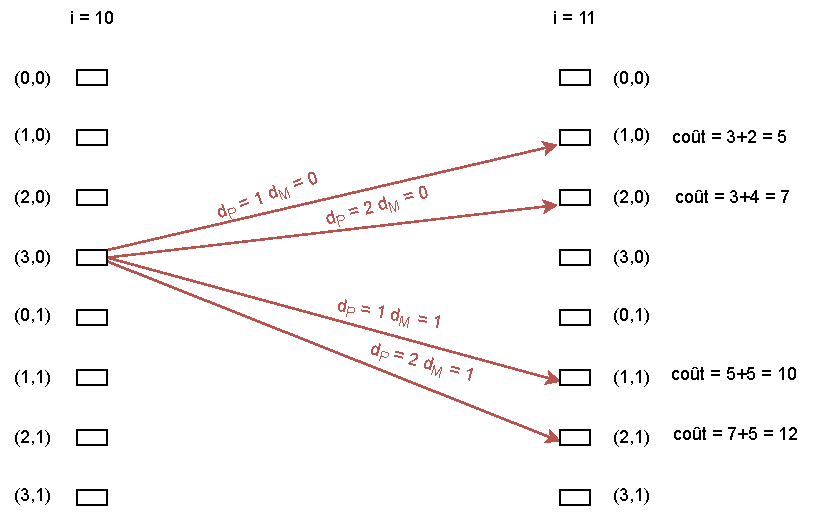
\includegraphics[height=9cm]{images_these/Arcs_associe.pdf}}
	\caption[Arcs associés aux Transitions]{Arcs associés aux Transitions dans le Réseau d'États associé à l'Exemple Production. }
	\label{Arcs_associe}
\end{figure}

La figure (\ref{Structure_G}) montre la structure générale du réseau des états, associé ici à $\mathcal{T}$ et $E$.
\begin{figure}[H]
	\centerline{
		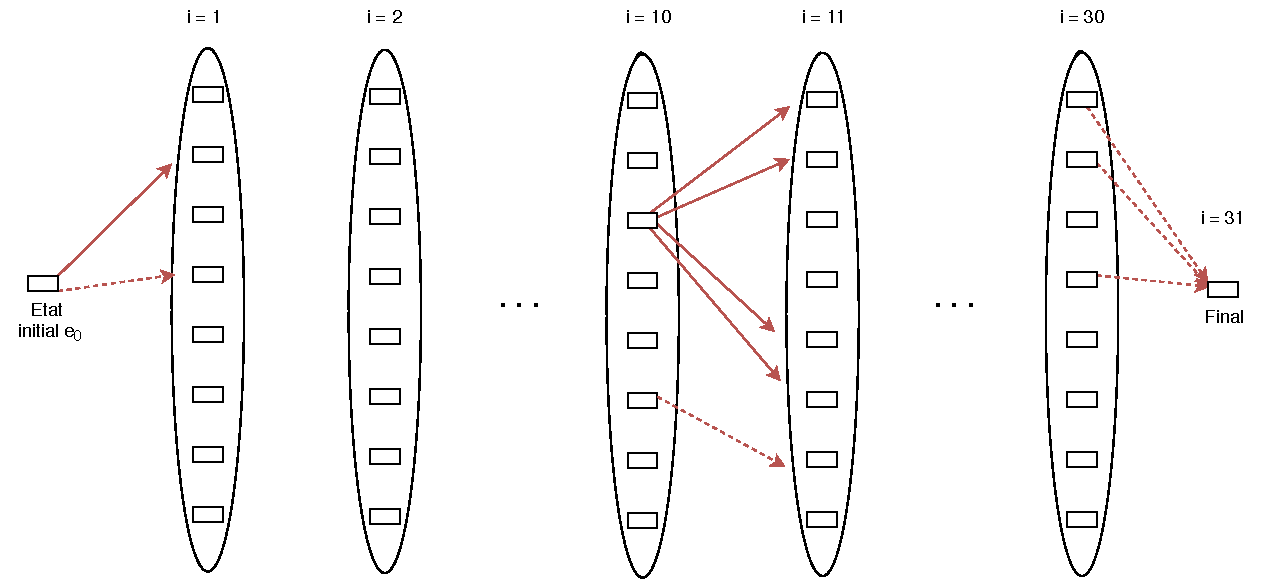
\includegraphics[height=9cm]{images_these/Structure_G.pdf}}
	\caption[Structure Générale du Réseau d'État "Production" ]{Structure Générale du Réseau d'État «Production».}
	\label{Structure_G}
\end{figure}

\textbf{Mesure de Performance et Principe de Bellman} : C'est un des points clés de la \textbf{PD} : une trajectoire au sens précédant est donc une suite de transitions $\Gamma = {(t_0, e_0), \dots, (t_{Fin}, e_{Fin})}$. %(ou bien une fonction $t \rightarrow e(t)$ dans le cas continu).
 A chaque transition ($(t, e) \rightarrow_d (t', e')$) de $TR$, il doit être possible d'associer une mesure de performance $Perf\_Trans((t, e) \rightarrow_d (t', e'))$. \textbf{La mesure de performance de la trajectoire doit dès lors pouvoir s'exprimer} $Perf(\Gamma) = \otimes Perf\_Trans((t_i, e_i) \rightarrow_{di} (t_{i+1}, e_{i+1}))$, où $\otimes$ désigne un opérateur associatif (en général le $+$, mais pas forcément, voir par exemple les algèbres dites exotiques en automatique). 
%Dans le cas continu, cette formule prendra une forme intégrale.
 Si on interprète l'ensemble des couples $(t, e)$ comme l'ensemble des nœuds d'un graphe orienté, alors la notion de trajectoire coïncide dans le cas déterministe et discret avec celle de chemin, et, quand l'opérateur $\otimes$ est l'opérateur $+$, celle de performance avec celle de longueur de ce chemin. 

C'est cette forme particulière de la mesure de performance d'une trajectoire qui fournit ce qu'on appelle le principe de Bellman. Dans le cas déterministe et discret, on va pouvoir noter $W(t, e)$, la performance optimale pour une trajectoire partielle aboutissant à l'instant $t$ sur l'état $e$,  et on aura alors : (\textbf{Equation Récursive de Bellman})

$W(t, e) = Sup_{Transitions\_possibles ((t' e') \rightarrow_{d} (t, e))}   [W(t', e') \otimes Perf\_Trans((t', e') \rightarrow_{d} (t, e))]$.

Les choses sont plus compliquées dans le cas stochastique ou encore dans le cas cyclique. On verra sur des exemples comment les choses peuvent alors se traiter. 

\textbf{Dans le cas de notre exemple}, la performance devient un coût, qu'il faut minimiser. Dans la formule ci-dessus, il faut donc remplacer Sup par Inf, l'opérateur $\otimes$ devenant de façon classique l'opérateur $+$. Le coût de la transition $((e_S, e_M) \rightarrow_{d} (e'_S, e'_M))$, réalisée entre $i$ et $i+1$ va être :
 
$Cout\_Transition = Cout\_Stock + Cout\_Prod + Cout\_Machine$ avec : 

\begin{itemize}[label=$\square$]
	\item	Si $d_P = 0$ alors $Cout\_Prod = 0$ sinon $Cout\_Prod  = Fix\_Prod_i + d_P \times Var\_Prod_i$ ; 
	\item	Si $(e_S + d_P - L_i ) = 0$ alors $Cout\_Stock = 0$ sinon  $Cout\_Stock = (e_S + d_P - L_i ) \times Var\_Stock +  Fix\_Stock$ ; 
	\item	$Cout\_Machine = (1 - e_M) \times d_M \times Install_i  + e_M \times Loc_i$.
\end{itemize} 

\textbf{Stratégie d'Implémentation du Principe de Bellman} : Concevoir un algorithme de Programmation Dynamique consiste donc à implémenter le \textit{Principe Récursif de Bellman}, tel que décrit ci-dessus. Suivant le cas, on pourra se projeter en avant (\textit{Forward Driven}) à partir de l'état initial ou au contraire en arrière (\textit{Backward Driven}) depuis les états finaux possibles, en encore adopter une stratégie mixte, dite \textit{Forward/Backward}, de façon à réduire le nombre des états créés. Il est cependant important de noter que des considérations autres qu'algorithmiques peuvent présider au choix d'une telle stratégie. Dans un certain nombre de cas, et notamment dans le cas des applications temps réel, l'algorithme PD n'est appliqué qu'en pré-\textit{process}, de façon à obtenir, pour chaque couple $(t, e)$, la décision optimale $d(t, e)$ associée. Cette décision est alors stockée dans une forme de table, et c'est la procédure de récupération en temps réel de cette décision qui est alors exécutée à chaque instant au fur et à mesure que la trajectoire se déroule. Outre la réactivité que cette façon de procéder apporte, celle-ci permet aussi de gérer les éventuelles perturbations, c'est-à-dire le fait que les transitions puissent induire des marges d'erreurs. Mais elle implique une implémentation \textit{Backward} du principe de Bellman, puisque c'est celle-ci qui va nous permettre de récupérer les décisions souhaitées :
 
\textit{\textbf{Equation Récursive de Bellman, en Forme Backward}} : Pour tout couple $t, e$, on note $V(t, e)$ la valeur de performance optimale d'une séquence de transitions permettant de connecter l'état $e$ à l'instant $t$ à un état final à l'instant final $N$. On obtient alors :
   
\begin{itemize}[label=$\square$]
	
	\item 	$V(t, e) = Sup_{Transitions\_possibles ((t, e) \rightarrow_{d} (t', e')}  [V(t', e') \otimes Perf\_Trans((t, e) \rightarrow_{d} (t', e'))] $ ;
	\item 	Décision associée $d(t, e) =$ Arg Sup.
\end{itemize}
 
\textbf{Dans le cas de notre exemple}, une implémentation Backward du principe de Bellman se fera en construisant, pour $i = N+1, N,\dots, 1, 0$, une liste $E(i)$ des états associés à l'instant $i$, dont chaque élément est constitué de :


\begin{itemize}[label=$\square$]
	\item 	Un état $e $ (état à l'instant $i$) ;
	\item 	Une valeur associée $V$, nulle dans le cas où $i = N+1$ ;
	\item 	Une décision associée $d$, prise à l'instant $i$, dans l'état $e$ et indéfinie dans le cas où $i = N+1$ ;
	\item 	Un pointeur $pt$ sur l'élément de la liste $E(i+1)$, qui correspond au résultat de la transition induite par $d$ depuis $(i, e)$.
\end{itemize}
Le processus fonctionnera alors comme décrit à l'algorithme (\ref{Backward-DPS Processus }).

\begin{algorithm} 
	\caption{Backward\_DPS }
	\label{Backward-DPS Processus }
	\begin{algorithmic}[1]
		%\REQUIRE
		%\ENSURE 
		%\hline
		%\vspace{0.5cm}
		%\INITIALISATION
		\STATE Initialiser $E(N+1) \leftarrow \{(e_f, 0, Indéfini, Nil)\}$ ; 
		%\vspace{0.3cm}
		%\BOUCLEPRINCIPAL
		\vspace{0.2cm}
		\FOR{$i=N$ \TO 0}
		\FOR{$(e',V',d',pt')$ dans $E(i+1)$}
		\STATE Générer les états $e$ et les décisions $d$ tels que la transition $(e \rightarrow_{d} e')$ est réalisable ;
		\FOR{tout couple $(e,d)$ ainsi généré}
		\IF{$e$ n'apparait pas dans $E(i)$ }
		\STATE insérer $(e, V, d, pt)$ dans $E(i)$ avec $V = V' + Cout\_Transition((i, e) \rightarrow_{d} (i+1, e'))$ et $pt =$ Pointeur sur $(e', V', d', pt')$ dans $E(i+1)$ ;
		\ELSE
		\STATE Soit $(e, V^*, d^*, pt^*)$ l'élément mettant en jeu $e$ dans $E(i)$ ;
		\IF{$V = V' + Cout\_Transition((i, e) \rightarrow_{d} (i+1, e')) < V*$ }
		\STATE Remplacer $V^*$ par $V$, $d^*$ par $d$ et $pt^*$ par $pt =$ Pointeur sur $(e', V', d', pt')$ dans $E(i+1)$; 
		\ENDIF
		\ENDIF
		\ENDFOR
		\ENDFOR
		\ENDFOR	
	\end{algorithmic}
\end{algorithm}

\textbf{	Filtrage } : Comme évoqué plus haut, une des difficultés majeures à traiter quand on cherche à implémenter un algorithme \textbf{PD} est liée à l'explosion potentielle du nombre des états. Se pose alors la question du \textbf{Filtrage}, c'est-à-dire des procédés susceptibles d'anticiper les états les plus pertinents. On distinguera quatre grandes classes de filtrage : 

\begin{itemize}[label=$\square$]
	\item	 \textit{Les filtrages par dominance} : On définit, soit de façon mathématiquement fondée, soit de façon heuristique
	%(NS meilleurs états)
	, un procédé de \textit{comparaison qualitative} des états, qui induit en général une relation d'ordre sur $E$, et ne conserve parmi les états générés pour une valeur $t$ donnée, que les états maximaux ou presque maximaux pour ce procédé.
	\item		\textit{Les filtrages par équivalence ou rounding} : On définit un procédé qui consiste à considérer comme équivalents entre eux deux états $e_1$ et $e_2$ « Proches ». On ne conserve alors, parmi les états générés pour une valeur $t$ donnée, qu'au plus un état par classe d'équivalence induite par ce procédé.
	\item		\textit{Les filtrages par anticipation logique} : On se dote de procédés de déduction (similaire à ceux utilisés pour la \textit{Propagation de Contraintes}), permettant d'anticiper que, à un instant donné $t$, il ne sera pas possible de prolonger (vers l'état final si on est en \textit{Forward} et vers l'état initial si on est en \textit{Backward}) un certain état $e$ en une trajectoire $\Gamma$ satisfaisant toutes les contraintes du problème. 
	\item	\textit{Les filtrages par estimation optimiste} : On se dote d'un procédé fournissant, pour tout couple $(t, e)$, une \textit{estimation optimiste} $Val(t, e)$, (en général une borne supérieure) de la meilleure performance possible pour une trajectoire partielle $\Gamma(e, t)$, démarrant en $(e, t)$ et se poursuivant jusqu'à un état final possible (si on est en \textit{Forward} et terminant en $(e, t)$ si on est en \textit{Backward}). Dès lors, pour peu que l'on ait été capable de pré-calculer de façon heuristique une trajectoire réalisable de valeur $WCour$, on peut appliquer le filtrage suivant : 
	\begin{itemize}
	\item si $(t, e)$ est tel $W(t, e) \otimes Val(t, e) \leq VCour$, $W(t, e)$ désignant la valeur associée à $(t, e)$ au sens de la formule de Bellman déclinée \textit{Forward},  alors tuer $e$ en tant qu'état possiblement associé à $t$.
	\end{itemize}
	Remarquons au passage que le fait de disposer du procédé d'estimation optimiste $Val$ permet de transformer de façon naturelle le schéma \textbf{PD} \textit{Forward} en un algorithme glouton, en implémentant le processus suivant :
	\begin{itemize}
	\item $(t, e) \leftarrow (t_0, e_0)$ ; 
	
	\item Tant que $(t, e)$ ne correspond pas à un état final faire :
	\begin{enumerate}
		\item Calculer une décision $d$ telle que $W(t, e) \otimes Perf\_Trans((t, e) \rightarrow_{d} (t', e')) \otimes Val(t', e')$ soit maximal;
		
		\item $(t, e) \leftarrow Etat (t', e')$ résultat de l'application de $d$ à $(t, e)$.
	\end{enumerate}
\end{itemize}
\end{itemize}

\textbf{Dans le cas de notre exemple}, on voit que la structure des états est très simple, essentiellement parce qu'on considère un seul produit \textit{output} et que l'on ne s'intéresse pas aux produits \textit{input}, et que l'on gère une production agencée de façon séquentielle dans le temps, chaque opération de production se déroulant sur une seule période $i$. Malgré cela on peut être confronté à un nombre important d'états pour peu que les unités utilisées pour mesurer production et stockage soient fines, et donc que l'espace des valeurs pour les variables $e_P$ et $d_P$ soient grands. Les notions évoquées ci-dessus pourront alors s'exprimer comme suit (on suppose que l'on se place dans l'hypothèse d'un parcours \textit{Forward}) :
\begin{itemize}[label=$\square$]
	\item	\textit{Filtrage par Dominance} : pour un instant $i$ considéré, on ne voit pas comment de façon mathématique dire qu'un état $e = (e_S, e_M)$ accompagné d'une valeur $W$, est meilleur qu'un état $e^* = (e^*_S, e^*_M)$ accompagné d'une valeur $W^*$. En effet, le fait de disposer de la machine ou d'un stock élevé n'est pas forcément un avantage, puisqu'il faudra payer pour les coûts de location et stockage induits. Toutefois, on peut considérer, de façon empirique,  que si la demande à fournir entre $i$ et $N$ est élevée et si les coûts de stockage sont faibles en comparaison des coûts de production, alors le fait d'avoir $e^*_M \geq e_M$, $W^* \leq W$ et $(e^*_S - e_S)$ au moins égal à un certain seuil rend un élément $(e^*, W^*, d^*, pt^*)$ de $E(i)$ meilleur que l'élément $(e, W, d, pt)$. On retire (tue) alors ce dernier de $E(i)$. 
	\item	\textit{Filtrage par Rounding} : Il suffit ici de changer d'unité de mesure des produits (par exemple, de compter en tonnes au lieu de compter en kilos. On se fixera donc un nombre de digits $K$ et considèrera que si $(e^*, W^*, d^*, pt^*$) et $(e, W, d, pt)$ dans $E(i)$ sont tels que $e_M = e^*_M$, $e_S = e^*_S$ et $W = W^*$ au $K$ plus grands digits, alors ils sont équivalents. On en supprimera donc un des deux.
	\item	\textit{Filtrage par Anticipation Logique} : La puissance d'un tel filtrage dépend, comme en programmation par contrainte, de l'habileté du programmeur à se projeter en avant. Il existe donc autant de procédés que de programmeurs habiles. De façon extrêmement rustique, on pourra remarquer ici que si à un instant $i$ donné, la somme $\sum_{ j \geq i} L_j$ des livraisons à effectuer est strictement plus grande que la capacité de production restante augmentée du stock courant, soit $(N- i+ 1)$$\times$ $C^{Prod\_Sup} + e_S,$ alors il ne sera pas possible de prolonger l'état $e$ à l'instant $i$ en une solution de notre problème. On pourra donc tuer le composant $(e, W, d, pt)$ associé dans $E(i)$.
	\item	\textit{Filtrage par Estimation Optimiste} : Il en est de même que pour les filtrages par anticipation logique. Leur puissance dépend de la capacité du programmeur à concevoir un procédé d'estimation $Val(t, e)$ qui fournisse une bonne approximation du coût à consentir afin de prolonger un état $e$ à un instant $t$ en une trajectoire complète. Ici, on pourra toujours remarquer (là encore de façon très rustique), que si on est dans un état $(e_S, e_M)$ à un instant $i$, et si $L = \sum_{ j \geq i} L_j$ est la quantité demeurant à livrer, alors il faudra produire au moins $(L -  e_S)$ quantité de produit, sur au moins $\lceil (L -  e_S)/ C^{Prod\_Sup}\rceil$ journées. Le coût induit sera donc au moins égal à $Val(i, e)  = (Inf_{j \geq i} Fix\_Prod_j) \times \lceil(L - e_S)/ C^{Prod\_Sup}\rceil  + (Inf_{j \geq i} Var\_Prod_j)\times (L -  e_S)$. Il faudra toutefois chercher quelque chose de plus sophistiqué si on veut vraiment obtenir un effet de filtrage conséquent.
	
\end{itemize}

\subsection{Exemples Simples}
\label{Exemples_Simples}
On va à présent illustrer ces notions générales au travers d'un certain nombre d'exemples, simples dans un premier temps (Section \ref{Exemples_Simples}), puis plus complexes (Section \ref{Le_Cas_Stochastique},  \ref{Le_Cas_Cyclique}) et traitant notamment du cas stochastique (Section \ref{Le_Cas_Stochastique}), %du cas continu (Section \ref{Le_Cas_Continu}), \ref{Le_Cas_Continu}, \ref{Jeu_de_Poursuit},
% du cas des Jeux (Section \ref{Jeu_de_Poursuit}) 
 et du cas cyclique (Section \ref{Le_Cas_Cyclique}).
\subsubsection{Le problème du sac à dos : Principe des FPTAS}
Le problème du sac à dos consiste en la recherche d'un vecteur $x = (x_1, \dots, x_N)$ à valeur en $\{0, 1\}$ et tel que :
\begin{itemize}[label=$\square$]
	\item	$\sum_i A_i \times x_i \leq B $;
	\item	il faut maximiser $\sum_i Ci\times x_i$.
\end{itemize}

Les coefficients entiers  $A_i$ , $C_i$ , $i = 1, \dots, N$, et $B$ sont donnés en entrées.

On notera qu'aucune notion évidente de temps n'est présente dans cet exemple, qui ne concerne pas un système dynamique. Pour autant, un espace-temps artificiel s'impose, qui est l'espace $\mathcal{T} = \{1, \dots, N, N+1\}$. 

L'espace d'état associé est alors l'espace $E$ des valeurs entières $ e$ entre $0$ et $B$. Sa signification est la suivante : à l'instant $i = 0, \dots, N+1$,  on a décidé des valeurs $x_j$, $j < i$, et la somme $\sum_{ j < i} A_j \times x_j$ vaut $e$. On doit alors décider de la valeur $x_i$.

L'état initial correspond à $i = 1$ et $e = 0$. Les états finaux correspondent à $i = N+1$ et $e \leq B$.
Les nœuds du réseau sans circuit associés à ces couples Temps/Etats sont formés de tous les couples $(i, e)$ ainsi obtenus. La figure \ref{Etats_Knapsack} explicite le passage des nœuds du réseau des états du problème du sac à dos associés à $i = 3$ à ceux associés à $i = 4$, quand $B = 100$, $A_3 = 5$, $C_3 = 4$.
% : Voir figure (\ref{Etats_Knapsack})

\begin{figure}[H]
	\centerline{
		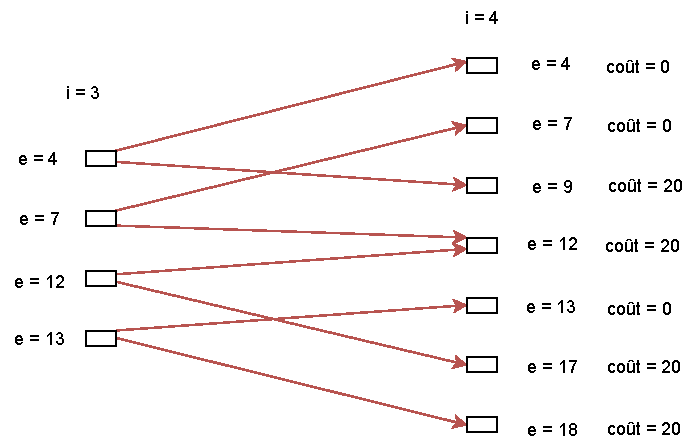
\includegraphics[height=9cm]{images_these/Etats_Knapsack.pdf}}
	\caption[Les nœuds du Réseau des Etats du problème du sac à dos. ]{Les nœuds du Réseau des Etats du problème du sac à dos.}
	\label{Etats_Knapsack}
\end{figure}

Une décision prise à l'instant $i$ depuis l'état $e$ porte sur la valeur $x_i$. Elle est réalisable si $e + A_i \times x_i \leq B$. La transition (arc du réseau) induite fait passer de $i$ en $i+1$ et de $e$ à $e + A_i\times x_i$. Son profit est $C_i\times x_i$. On retient, parmi les états finaux possible $e$, celui qui est associé à la plus grande valeur de profit cumulé $w$, qui constitue donc la valeur optimale $V^{Opt}$ de notre problème du sac à dos.

L'algorithme de \textbf{PD}, que l'on notera \textbf{PD-Knap}, qui en découle n'est pas polynomial (on sait que le problème du sac à dos est NP-Difficile) : en effet le nombre d'états à priori possibles est $B$, et est donc en $2^{k(B)}$, où $k(B)$ est la taille de codage de l'entier $B$. Il est toutefois presque polynomial : si l'on limite les valeurs de B de telle sorte qu'elles n'excèdent une valeur $Q(N)$, où $Q$ est un polynôme, alors on voit que cet algorithme devient polynomial. Cela suggère à rendre notre algorithme presque polynomial, en arrondissant les valeurs prises par les états $e$, de telle sorte que leur nombre demeure polynomial en fonction de $N$, quitte à consentir une marge d'erreur sur le résultat final. C'est le sens de ce qu'on nomme les \textbf{PTAS} (\textbf{Polynomial Time Approximation Scheme}).

Construire un \textbf{PTAS} (\textbf{Polynomial Time Approximation Scheme}) consiste à construire un algorithme paramétré, qui une fois la valeur du paramètre fixée, devient polynomial au sens du temps, modulo un certain niveau d'approximation. On va jouer ici sur les tailles de codage et transformer l'algorithme \textbf{PD-Knap} ci-dessus comme suit :

\begin{itemize}[label=$\square$]
	\item	On se fixe un nombre $K$, qui est un nombre de bits.
	\item	Pour chaque nombre entier $p$, dont l'écriture en base 2 est $\sum_{j = 0,\dots,k(p)} u_j\times 2^j$, on pose $Round(K, p) = \sum_{j = k(p) - K+1 ,\dots,k(p)} u_j \times 2^j$,  c'est-à-dire que l'on ne garde de $p$ que ses $K$ bits les plus élevés (on dit aussi que l'on arrondit aux $K$ plus grands bits). On dit que 2 couples $(a, w)$ et $(a', w')$ de nombres entiers sont alors équivalents modulo les $K$ plus grands bits si $Round(K, a) = Round(K, a')$ et $Round(K, w) = Round(K, w')$.
	\item	On adapte alors le schéma \textbf{PD} précédant en gardant l'espace temps $\mathcal{T} = {1, \dots, N+1}$ et en prenant comme espace d'état $E$ l'ensemble des couples $e = (a \leq B, w)$ : à chaque instant $i$, on a décidé des valeurs $x_j$, $j < i$, la somme $\sum_{j < i } A_j\times x_j$ vaut $a$ et la somme $\sum_{j < i} C_j\times x_j$ vaut $w$.  On doit alors décider de la valeur $x_i$. La décision $x_i$ étant choisie, on passe alors (transition) à l'instant $i+1$ dans l'état $e' = (\sum_{j \leq i} A_j \times x_j, \sum_{j \leq i} C_j\times x_j)$. On exige que $\sum_{j \leq i} A_j\times x_j \leq B$.
	\item	Durant le passage $i \rightarrow i+1$, on applique le filtrage suivant : 
	\begin{itemize}
		\item	On implémente \textbf{PD} selon la stratégie \textit{Forward} ;
		\item	On fait en sorte, que, dans l'espace $E(i+1)$ des états associés à l'instant i+1 à l'issue du passage $i \rightarrow i+1$, \textbf{il n'y ait pas 2 états $e'$ et $e''$ qui soient équivalents modulo les $K$ plus grands bits}.  Si, à partir de $E(i)$,  on a fait apparaitre $e'$ et $e''$ équivalents modulo les $K$ plus grands bits, alors \textbf{on élimine celui qui a le plus grand composant} $a = \sum_{j \leq i} A_j \times x_j$. 
	\end{itemize}
	\item	On retient, parmi les états $(a, w)$ obtenus avec $i = N+1$, celui qui correspond à la plus grande valeur $w$, qui fournit donc la valeur de l'algorithme.
\end{itemize}
On obtient ce faisant, un algorithme paramétré par le nombre $K$. On le note \textbf{PD-Knap}($K$). Si $K$ est fixé, cet algorithme devient polynomial au sens temps, puisque le nombre d'éléments dans chaque ensemble $E(i)$ ne peut excéder $2^{2K} \times (k(B) - K +1)\times (k(C) - K +1)$, où $C = \sum_i C_i$.  En même temps, on peut rendre cet algorithme aussi proche de l'optimalité que l'on veut en augmentant le nombre $K$.

La figure (\ref{Regroupement_Etats}) explique comment on regroupe ainsi les états par classe d'équivalence modulo les $K = 3$ plus grands bits :

\begin{figure}[H]
	\centerline{
		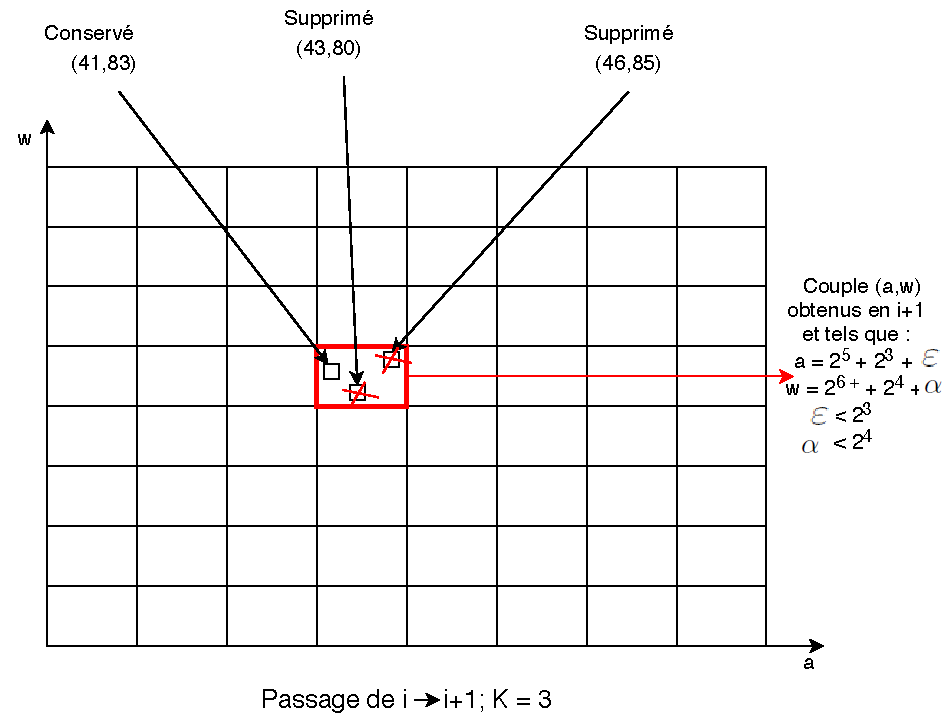
\includegraphics[height=10cm]{images_these/Regroupement_Etats.pdf}}
	\caption[Regroupement des états. ]{Regroupement des états $(a, w)$ par classe d'équivalence modulo les 3 plus grands bits.}
	\label{Regroupement_Etats}
\end{figure}

\begin{theo}{\textbf{PTAS du Sac à dos}}
	\label{dem_PTAS}
	%Soit un petit nombre $\varepsilon > 0$, et soit $V^{Opt}$ la valeur optimale de notre problème de Sac à dos. On peut choisir $K_0$ tel que pour tout $ K \geq K_0$,  l'algorithme \textbf{PD-Knap}($K$) calcule une solution réalisable $x$ dont la valeur $V(K)$ est telle que l'erreur relative $(V^{Opt} - V(K))/V^{Opt}$ est au plus égale à $\varepsilon$. 
	
	Pour tout $\varepsilon > 0$, on peut concevoir un algorithme $P^{\varepsilon}$ tel que pour toute instance $I$ de valeur optimale $V^{Opt}$ de notre problème du Sac à dos on ait :
	\begin{itemize}[label=$\square$]
		\item $P^{\varepsilon}$ calcule une solution réalisable $x$ de valeur $V$ de $I$ en temps polynomial ;
		\item Le quotient \og Erreur relative commise par $P^{\varepsilon}$ \fg{}  ${\displaystyle {\frac {V^{Opt}-V}{V^{Opt}}}} \leq \varepsilon$.
		\end{itemize}
	
\end{theo}
%La démonstration de ce théorème se trouve en annexe à la section \ref{dem_PTAS_section}.


\subsubsection{Le \textit{Split}}

On parle de procédé \textit{Split} quand on cherche à partitionner une liste $L$ en sous-listes $L_1, \dots, L_Q$,  constituant chacune un segment de $L$ (constituée d'éléments consécutifs dans $L$), de façon à minimiser un coût défini par les jointures entre les différentes listes. Il est utilisé en algorithmique des problèmes dits de Tournées de Véhicules, quand on cherche à distribuer une liste de clients $L$ (notion de tour géant) donnés dans un certain ordre, entre des véhicules qui assureront le service d'un sous-ensemble de clients consécutifs au sens de $L$.

Différentes variantes du \textit{Split} existent, plus ou moins complexes selon que l'on envisage ou non différentes catégories et suivant la façon dont on définit les coûts. On va prendre ici le cas le plus simple, sachant que, dans tous les cas, l'algorithmique du \textit{Split} reste sensiblement le même.

Considérons donc notre liste $L$, que l'on peut imaginer comme un tour $\{0 = Depot, 1, 2, \dots, N, N+1 = 0 = Depot\}$ réalisé par un véhicule unique, partant d'un Dépôt nommé $Depot$ et visitant dans cet ordre des clients $i = 1, \dots, N$, avant de revenir au Dépôt. Cet ensemble $X = \{0, 1, \dots, N\}$ est muni d'une distance : $D_{i,j}$ désigne la distance de $i$ à $j$. A chaque client $i$ correspond une charge $C_i$. Un nombre $K$ étant donné, on cherche alors à distribuer ces clients entre $K$ véhicules identiques, de capacité $CAP$, de façon à ce que les contraintes de capacités ne soient pas violées et que :
\begin{itemize}[label=$\square$]
	\item	Problème \textbf{SplitMax} : le Max des temps de parcours des véhicules soit le plus petit possible ;
	\item	Problème \textbf{SplitSum} : la somme des temps de parcours des véhicules soit la plus petite possible.
\end{itemize}	
	Dans les deux cas, notre espace-temps va être l'espace ordonné ${0, 1, \dots, N, N+1}$ et l'espace $E$ des états va être composé des valeurs $e = 0, 1, \dots, K$, avec, pour un tel état $e$ associé à un instant $i$,  la signification suivante :
\begin{itemize}[label=$\square$]
	\item	On a traité tous les clients $j$ tels que $1 \leq j \leq i$ (si $i = 0$ il n'y a pas de tels clients), et cela en utilisant $e$ véhicules. Si $i \leq N$ on doit avoir $e \leq K-1$.
	\item	L'état initial $e_0$ est bien sûr $e_0 = 0$ ; L'état final est tout e associé à $N+1$ et tel que $e \leq K$.
\end{itemize}
	Une décision est alors définie par un indice $j$ tel que : $i+1 \leq j \leq N+1$, tel que : 
	\begin{itemize}[label=$\square$]
		\item	$\sum_{i+1 \leq q \leq j} C_q \leq CAP$ ; (on pose $C_0 = C_{N+1} = 0$)
		\item	Si $e = K-1$ alors $j = N+1$ ;
	\end{itemize}
	La transition induite va de $(i, e)$ à $(j, e+1)$. Son coût est $D_{Depot,i+1} + \sum_{i+1 \leq q \leq j-1} D_{q,q+1} + D_{j,Depot}$ .
	
	Le distinguo entre \textbf{SplitMax} et \textbf{SplitSum}, se trouve au niveau de l'opérateur associatif $\otimes$ qui combine les coûts des différentes transitions aux fins d'obtenir un coût cumulé. Dans le premier cas, $\otimes$ est l'opérateur Max, et dans le deuxième, il s'agit classiquement de l'opérateur $+$. Dans ce dernier cas aussi, on voit que l'on peut simplifier la spécification du coût des transitions en ne tenant compte que des détours induits par le changement de véhicule, c'est-à-dire des termes$D_{Depot,i+1} + D_{j,Depot}$ .



\subsection{Le Cas Stochastique}
\label{Le_Cas_Stochastique}

Il est au cœur de nombreuses situations réelles, notamment celles liées à la gestion d'actifs financiers. Nous n'allons faire ici que l'effleurer, de façon à en faire percevoir la complexité.

Reprenons l'exemple de la Section (\ref{Cadre_general}) et lié à la gestion de production. Dans la plupart des situations concrètes, il existe des incertitudes quant à la fraction d'objets produits qui ne pourront être livrés du fait de défauts, et, surtout, quant à la demande. Même quand les demandes sont associées à des commandes, celles-ci peuvent être annulées ou reportées, ou au contraire, des demandes non prévues peuvent apparaitre qui nécessitent une certaine réactivité de la part de l'entreprise. Dans notre cas, on peut imaginer que, pour chaque jour $i = 1, \dots, N$, la demande $L_i$ soit incertaine, et qu'une analyse statistique des historiques permette de quantifier cette incertitude sous forme probabiliste : pour chaque $i$, $L_i$ devient une distribution de probabilité à l'intérieur d'un espace $D_i$ de valeurs possible de demandes pour le soir $i$. Par exemple, pour le jour $i = 10$, on pourra supposer que $D_i = \{4, 5, 6\}$ et que $L_i$ est la distribution de probabilité $\{1/4, 1/2, 1/4\}$. On supposera aussi $Fix\_Prod_{10} = 10$, $Var\_Prod_{10} = 4$,  $Fix\_Stock = 1$, $Var\_Stock = 1$.

\subsubsection{Un Premier Niveau de Difficulté : Intégrer dans le Modèle le Comportement du Système Réel face aux aléas}
\label{Premier_Niveau_de_Diff}
Conceptuellement, l'introduction du non déterminisme signifie qu'à une décision donnée correspond, non pas une transition unique, mais plusieurs, subordonnées à l'évènement \og demande en $i$ \fg{} $d \in D_i$ (voir Figure \ref{arc-transition}). Si, par exemple, on est dans un état $(e_S = 3, e_M = 0)$, et que l'on prend une décision $(d_P = 2, d_M = 0)$, alors cette décision est susceptible d'avoir trois résultats possibles à l'instant $i+1$ :
\begin{itemize}[label=$\square$]
	\item	Avec probabilité $1/4$ : le stock résultant est 1 : le coût de production induit est 18, le coût de stockage induit est 2 ;
	\item	 Avec probabilité $1/2$  : le stock résultant est 0 : le coût de production induit est 18, le coût de stockage induit est 0 ;
	\item	Avec probabilité $1/4$ : le stock résultant est 0 : le coût de production induit est 18, le coût de stockage induit est 0, mais, on a été incapable de satisfaire une demande. 
\end{itemize}
\begin{figure}[H]
	\centerline{
		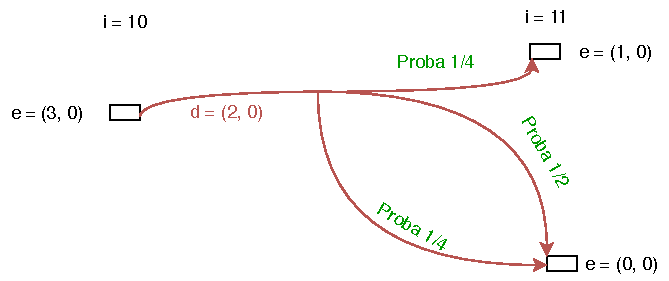
\includegraphics[height=6cm]{images_these/arc-transition.pdf}}
	\caption[Un arc-transition non déterministe. ]{Un arc-transition non déterministe.}
	\label{arc-transition}
\end{figure}

Supposons maintenant que l'on a une capacité de stockage de 4, et que par souci d'anticipation des coûts favorables, on ait décidé de produire $d_P = 6$. Alors on n'a plus de problème de demande non satisfaite, mais on a \textbf{un excès de stock} dans le cas (Avec probabilité 1/4 ) ou la demande en $i$ est seulement de 4. Doit-on en déduire que la décision est forcément non réalisable ?

Cette première analyse fait apparaitre un premier niveau de difficulté : afin d'intégrer les incertitudes, on est amené à élargir le modèle, de façon à intégrer le fait que certaines contraintes du modèle déterministe (satisfaction des demandes ou des capacités) ne peuvent plus forcément être considérées comme des contraintes, sauf à rendre le modèle trop rigide, et doivent être aménagées de façon à coller avec la réalité du système :
\begin{itemize}[label=$\square$]
	\item	Demandes non satisfaites : on peut les ignorer, les décaler, ou au contraire les intégrer en tant que pénalités si on considère qu'elles induisent une perte d'image (difficile à quantifier) ;
	\item	Non respect des capacités de stockage : pratiquement, il faut regarder si ces contraintes sont « dures » (peut-on « faire de la place » ?), si il est possible de louer de la place de stockage additionnelle auprès d'un partenaire ($\Rightarrow$ coût additionnel), ou s'il faut détruire la production excédentaire (coût de destruction ?). 
\end{itemize}
La réponse à ces questions ne peut être fournie à partir du seul modèle déterministe, et exige un retour sur le terrain. 

\subsubsection{Un deuxième Niveau de Difficulté : La Problématique des Corrélations}
 \label{markov}
Supposons à présent que l'on ait réussi à contourner les obstacles soulevés à la section \ref{Premier_Niveau_de_Diff}, et donc que l'on ait fait en sorte que chaque décision admissible $d$ prise depuis un état $e$ à un instant $i$ induise une transition $TR$, pour laquelle chaque évènement $\omega$ induira à son tour un état $e'$ résultant $TR(i, e, \omega)$, selon un probabilité $P_\omega (e')$et un coût $ Cout\_TR(i, e, e')$. Si l'on se réfère à l'exemple de gestion de production, on peut imaginer avoir pénalisé, par un coût additionnel, toute demande non satisfaite ainsi que tout dépassement de capacité (ce qui revient à supprimer les capacités pour les remplacer complètement par des coûts). 

A ce moment là, on est en mesure d'implémenter un schéma \textbf{PD}, en se focalisant sur l'espérance (au sens probabiliste) du coût d'une stratégie de gestion : 
\begin{itemize}[label=$\square$]
	\item	On note, pour tout instant $i$, et tout état $e$ associé, $WP(i, e)$, l'espérance conditionnelle de Coût pour une trajectoire optimale débutant à l'instant $i$ et se finissant à l'instant $N$ final, et cela à partir de l'état $e$.  
	\item	On remarque alors que la seule stratégie de recherche possible pour l'implémentation d'une telle définition est la stratégie \textit{Backward}, qui seule permet de tirer partie de la façon dont les transitions sont probabilisées (depuis l'état de départ vers les états résultants).
	Pour tout instant $i$, tout état $e$ associé et toute décision  $d$, on peut écrire que, si l'on est en mesure d'appliquer la stratégie optimale associée à $WP$ à partir de tout instant ultérieur à $i$, alors le coût induit par la décision $d$ sera : $Cout\_Trajectoire(d, i, e) = \sum_{e'} P_\omega (e') \times (Cout\_Transition(((i, e) \rightarrow_{d,\omega} (i', e')) + WP(i', e'))) $. 
	
	Notre principe de Bellman s'adapte alors sans difficulté, sous la forme :
	
	\begin{itemize}[label=$\square$]
		
		\item	$WP(i, e) = Inf_{d}  Cout\_Trajectoire(d, i, e)  =  Inf_{d}   \sum_{e'} P_\omega (e') \times (Cout\_Transition(((i, e) \rightarrow_{d,\omega} (i', e')) + WP(i', e')))$. Où $d$ représente toutes les décisions possibles.
		\item	Décision associée $d(t, e) = Arg$ $Inf$.
	\end{itemize}
\end{itemize}

\textbf{Sur notre exemple} : Supposons que l'on soit en $i = 10$, dans un état $e =  (e_S = 1, e_M = 0)$, avec $D_i = \{3, 5, 7\}$, $L_i$ = $\{1/4, 1/2, 1/2\}$ la distribution de probabilité associée. On suppose  $Fix\_Prod_{10} = 10$, $Var\_Prod_{10} = 4$,  $Fix\_Stock = 1$, $Var\_Stock = 1$, ainsi qu'une capacité de stockage de 2. On a enfin convenu de pénaliser de 2 unité-coût/unité-stockée tout dépassement de capacité et de 3 unités-coûts/unité-demandée tout manquement à la demande. Si l'on prend alors la décision $(d_P = 4, d_M = 0)$, alors cette décision est susceptible d'avoir 3 résultats possibles à l'instant $i+1$ :
\begin{itemize}[label=$\square$]
	\item	Avec probabilité 1/4 : le stock résultant est 3 : le coût de production induit est 26, le coût de stockage (pénalisé) induit est 5 donc le Total est 31 ; Etat résultant $e_1 = (3, 0)$ ;
	\item	 Avec probabilité 1/2  : le stock résultant est 1 : le coût de production induit est 26, le coût de stockage induit est 2 donc le Total est 28 ; Etat résultant $e_2 = (1, 0)$ ;
	\item	Avec probabilité 1/4 : le stock résultant est 0 : le coût de production induit est 26, le coût de stockage induit est 0 ; la pénalité liée à la demande est 3 donc le Total est 29 ; Etat résultant $e_3 =  (0, 0)$.
\end{itemize}

Si l'on suppose que l'on a su calculer, pour i = 11, les valeurs $WP(11, e_1) = 108$,  $WP(11, e_2) = 111$, $WP(11, e_3) = 106$, alors on voit que $Cout\_Trajectoire(d, i, e) =  (31 + 108)/4 + (28+111)/2 + (29 + 106)/4 =  138$.

Mais une difficulté apparait alors :  La formule 

$Cout\_Trajectoire(d, i, e) = \sum _e' P_\omega (e') \times (Cout\_Transition(((i, e) \rightarrow_{d,\omega} (i', e')) + WP(i', e'))$  qui nous permet ce calcul repose sur l'hypothèse d'\textit{indépendance}. Les différents évènements susceptibles d'intervenir durant le processus doivent être \textit{indépendants} (ou Markovien ou \textit{sans mémoire}), ce qui permet d'écrire que si $P_A$ et $P_B$ sont les probabilités que 2 d'entre eux, $A$ et $B$, interviennent, alors la probabilité que les 2 interviennent au cours du même processus est égale au produit $P_A\times P_B$.  Cette hypothèse, présente aussi dans les modèles de gestion d'actifs financiers reposant sur le \textit{Mouvement Brownien}, facilite considérablement les calculs. Mais elle correspond rarement à la réalité, dans la mesure où elle nie la relation de causalité.  Dans le cas par exemple de notre système de production, le fait que la demande à l'instant 10 soit 3 plutôt que 5 peut avoir plusieurs causes : l'une d'entre elles est que la demande manquante est l'objet d'un délai, et qu'on va la retrouver à l'instant i+1 sous forme d'une augmentation de la demande prévue en 11 ; une autre, qui va en sens opposé, est que la demande a fléchi parce que le produit est apprécié de façon négative, ou parce qu'un produit concurrent moins cher (ou meilleur) est en train d'émerger, ou encore à cause de la conjoncture globale. Saisir ces causalités, et donc les \textit{corrélations} qui peuvent exister entre les distributions de probabilités $L_i$, est en soi difficile. Les intégrer à des calculs l'est encore plus. Une tendance actuellement est de remplacer des modèles basés sur des équations de type Bellman mettant en jeu ces hypothèses Markoviennes par des mécanismes d'apprentissage statistique exploitant des historiques. 
\poubelle{
\subsection{Le Cas Continu (Contrôle Optimal)}
\label{Le_Cas_Continu}

On considère donc ici l'espace-temps $\mathcal{T}$ comme étant continu. On va voir sur un exemple comment le principe de Bellman se décline sous forme d'équations différentielles, et comment le traitement de ces équations contraint à une stratégie \textit{Backward}. 

Prenons l'exemple suivant très ancien (Euler), de la \textit{Dolichobrachistochrone}. Il s'agit de la courbe $\Gamma$ que doit suivre un objet $ P$, pour rouler sans frottement en étant mû par la seule force de gravitation,  depuis un point donné $M_0$ de coordonnées $(1, H > 0)$ jusqu'au point $O = (0, 0)$, de façon à ce que le temps de parcours induit soit minimal (contrairement à ce que l'on pourrait penser, $\Gamma$ n'est ni une droite ni une parabole).

Notre objet va donc suivre une courbe $ t \rightarrow (x(t), y(t))$, et la loi de conservation d'énergie : $ m \times v^2/2 = m\times (H-y)\times g$, ou $v$ est la vitesse, $m$ la masse et $g$ le coefficient de force de gravitation,  permet d'écrire, à chaque instant $t$ : 
\begin{itemize}[label=$\square$]
	\item 	$(x'(t)^2 +  y'(t)^2) = 2\times (H-y(t))\times g$.
\end{itemize}
Si $\omega$ désigne l'angle entre le vecteur vitesse de notre objet à l'instant $t$ et l'axe des $x$, on obtient :
\begin{itemize}[label=$\square$]
	\item	$x'(t) = (2 \times (H-y(t)) \times g)^{1/2} \times cos(\omega)$ ;
	\item	$y'(t) = (2 \times (H-y(t)) \times g)^{1/2}  \times sin(\omega)$.
	
\end{itemize}

Afin de simplifier ces équations, et de rendre la progression de l'objet en avant plus lisible, on va :
\begin{itemize}[label=$\square$]
	\item	Changer d'unité de temps de façon à faire disparaitre le 2 et le $g$ ;
	\item	Changer d'unité d'espace de façon à remplacer $H$ par 1 ;
	\item	Considérer que l'instant final est l'instant $t = 0$, et donc que les valeurs t utilisées ici sont $\leq 0$ ;
	\item	Considérer que l'objet $P$ va en montant, depuis un point $(x_0 < 0, - 1)$ vers le point $(0, 0)$, ce qui nous permettra de manipuler des vecteurs vitesse orientés dans le sens des $x$ et des $y$ croissants.
\end{itemize}
Les équations (\ref{object_b_etat_art}) qui régissent alors le comportement de l'objet P sont :	


\begin{subequations}
	\label{object_b_etat_art}
	\begin{equation}
	dx/dt= x'(t) 	 = (1 + y)^{1/2}\times Cos(\omega(t)) 
	\end{equation}
	\begin{equation}
	dy/dt = y'(t)	 =  (1 + y)^{1/2}\times Sin(\omega(t))
	\end{equation}
\end{subequations}

On pose $H(y) = (1 + y)^{1/2}$, et on considère l'angle $\omega(t)$ comme paramètre de décision : on procède comme si un pilote était embarqué sur $P$ et tenait un volant qui lui permettait de choisir la courbe $\Gamma$ parcourue.  

Si l'on se réfère au schéma \textbf{PD}, on voit qu'un état de notre système est alors la position $(x, y)$ de l'objet $P$, et la décision devient l'angle $\omega$. On peut alors noter $V(x, y)$ la valeur, au sens programmation dynamique \textit{Backward}, associée à l'état $e = (x, y)$,  c'est-à-dire la temps minimal qu'il faut pour aller du point $(x, y)$ au point $O = (0, 0$) conformément aux équations (\ref{object_b_etat_art}). Si on est dans un tel état $e = (x, y)$ à un instant $t$, si on effectue un premier petit mouvement $t \rightarrow t + dt$, $(x, y) \rightarrow (x+ dx, y + dy)$ et qu'ensuite on continue en appliquant une stratégie optimale, alors le coût de la trajectoire induite sera : 

$Cout = dt + V(x+ dx, y + dy) = V(x, y) + [dt\times 1 + (\partial V/\partial x)\times dx + (\partial V/\partial y)\times dy]$. 

La décision optimale (principe de Bellman) est que $Cout$ sera minimal si la décision $\omega$ est tel que $[1 + ( \partial V/ \partial x)\times dx + ( \partial V/ \partial x)\times dx)]$ est minimal. Dans ce cas on aura $Cout = V(x, y)$. On devra donc avoir :

\textbf{Equation de Bellman} : $Inf_\omega [1\times dt + ( \partial V/ \partial x)\times dx + ( \partial V/ \partial y)\times dy)] = 0$.

On voit que :

$[1\times dt + ( \partial V/ \partial x) \times dx + ( \partial V/ \partial x)\times dx)] = 1\times dt + ( \partial V/ \partial x)\times H(y)\times Cos(\omega(t)\times dt  + ( \partial V/ \partial y)\times H(y)\times Sin(\omega(t)\times dt) = dt\times [ 1 +  ( \partial V/ \partial x)\times H(y)\times Cos(\omega(t)\times dt  + ( \partial V/ \partial y)\times H(y)\times Sin(\omega(t)]$.

L'\textbf{Equation de Bellman} se réécrit donc : 

$Inf_\omega [ 1 +  ( \partial V/ \partial x)\times H(y) \times Cos(\omega(t) + ( \partial V/ \partial y)\times H(y)\times Sin(\omega(t)] = 0$. Le Inf ci-dessus est obtenu pour :

\begin{itemize}[label=$\square$]
	\item	$Cos(\omega(t)) =  - ( \partial V/ \partial x)/(( \partial V/ \partial x)^2+ ( \partial V/ \partial y)^2)^{1/2} $; 
	\item	$Sin(\omega(t)) = - ( \partial V/ \partial y)/(( \partial V/ \partial x)^2+ ( \partial V/ \partial y)^2)^{1/2} $.
\end{itemize}
Afin d'avoir des notations plus fluides, on pose : 
\begin{itemize}[label=$\square$]
	\item	$V_x = V_x(x,y) = ( \partial V/ \partial x) $; 
	\item	$V_y= V_y(x,y) = ( \partial V/ \partial y) $;
	\item	$\Delta = \Delta(x,y) = (( \partial V/ \partial x)^2+ ( \partial V/ \partial y)^2)^{1/2}  = ((V_x)^2+ (V_x)^2)^{1/2} $.
\end{itemize}
On obtient alors : (\ref{object_b_etat_art})
\begin{itemize}[label=$\square$]
	\item	$dx/dt = - H(y)\times \Delta \times V_x$;
	\item $	dy/dt = - H(y)\times \Delta\times V_y$.
\end{itemize}
On a aussi (Bellman) : $[1 -  \Delta \times H(y)] = 0$, soit encore :

\begin{equation}
\label{belman_E2}
1 = \Delta^2 (1+y) = ((V_x)^2+ (V_x)^2)\times (1+y)
\end{equation}


On a un système de deux équations différentielles par rapport à la variable temps t, avec quatre inconnues $x$, $y$, $V_x$, $V_x$. Il nous faut donc deux équations supplémentaires que l'on obtient en dérivant l'équation (\ref{belman_E2}) de Bellman en $x$ et en $y$, et en remarquant que : 

\begin{itemize}[label=$\square$]
	\item$	dV_x /dt =  ( \partial^2V/ \partial x^2)\times (dx/dt) + ( \partial^2 V/ \partial y \partial x)\times (dy/dt) = ( \partial^2 V/ \partial x^2)\times (dx/dt) + ( \partial^2 V/ \partial x \partial y)\times (dy/dt) = ( \partial V_x/ \partial x)\times (dx/dt) + ( \partial V_y/ \partial x)\times (dy/dt)$
	
	\item	$dV_y/dt =  ( \partial^2 V/ \partial x \partial y)\times (dx/dt) + ( \partial^2 V/ \partial^2 y)\times (dy/dt) = ( \partial^2 V/ \partial y \partial x)\times (dx/dt) + ( \partial^2 V/ \partial^2 y)\times (dy/dt) = ( \partial V_x/ \partial y)\times (dx/dt) + ( \partial V_y/ \partial y)\times (dy/dt)$.
\end{itemize}
On déduit alors (calcul de routine) : 
\begin{itemize}[label=$\square$]
	\item	En dérivant (\ref{belman_E2}) en x : $dV_x /dt = 0 $;
	\item	En dérivant (\ref{belman_E2}) en y : $dV_y/dt = \Delta/2H(y)$.
\end{itemize}
On a alors un système différentiel complet sur $x$, $y$, $V_x$, $V_y$ en fonction de $t$ : (\ref{belman_E3})

\begin{subequations}
	\label{belman_E3}
	\begin{equation}
	dx/dt = - H(y) \times \Delta \times V_x
	\end{equation}
	\begin{equation}
	dy/dt = - H(y) \times \Delta \times V_y
	\end{equation}
	\begin{equation}
	dV_x /dt = 0 
	\end{equation}
	\begin{equation}
	dV_y/dt = \Delta/2H(y)
	\end{equation}
	
\end{subequations}

Il faut compléter ce système avec des conditions initiales, c'est-à-dire des conditions (Processus Backward) en $t = 0$, qui correspondent à la fin de trajectoire. On a $x(0) = y(0) = 0$. On ne connait ni $V_x(0)$ ni $V_y(0)$, mais on sait (Equation (\ref{belman_E2}) de Bellman) que quand $t \rightarrow 0$, $y \rightarrow 0$, et donc $(V_x)^2+ (V_x)^2 \rightarrow 1$, ce qui signifie que l'on doit pouvoir trouver un angle  $\alpha$  tel que : $V_x = Cos( \alpha)$ et $V_y = Sin( \alpha), \alpha \in [\Pi,3\times \Pi/2]$. Nos conditions initiales se retrouvent donc résumées par :		$(E4( \alpha ))$
\begin{itemize}[label=$\square$]
	\item $	x(0) = y(0) = 0 $;
	\item	$V_{x(0)} = Cos(\alpha)$ et $V_{y(0)}  = Sin(\alpha)$, $\alpha$ $\in$ [$\Pi, 3 \times \Pi/2$].
\end{itemize}
On touche ici un des points difficile du Contrôle Optimal. A chaque valeur de paramètre  $\alpha$ , va correspondre une trajectoire $\Gamma_\alpha$  qu'on pourra calculer par une méthode de \textit{Pas} classique, et deux trajectoires associées à des valeurs  $\alpha$  différentes seront disjointes (Voir Figure \ref{Deux_trajectoires}).  Si on se donne un point de départ $M_0 = (x_0, -1)$ il faudra alors déterminer le  $\alpha$  tel que  $\Gamma_\alpha$  contient $M_0$, ce qui peut constituer un problème difficile. Différentes techniques pourront être implémentées. L'une d'entre elles, particulièrement adaptée au contrôle de trajectoire en temps réel, consiste à résoudre (\ref{belman_E3}) et (E4( $\alpha$ )) pour un ensemble suffisamment dense de valeurs  $\alpha$  situées dans la zone probable pour   $\alpha$ , de stocker les résultats sous forme de nuages des points dans une table,  et, pour toute position $M$ courante, de procéder par interpolation (voir Figure \ref{Interpolation})à partir des positions dans la table les plus proches de $M$ afin d'en extraire la valeur $V$ et la décision $\omega$ \textit{ad hoc}.


\begin{figure}[H]
	\centerline{
		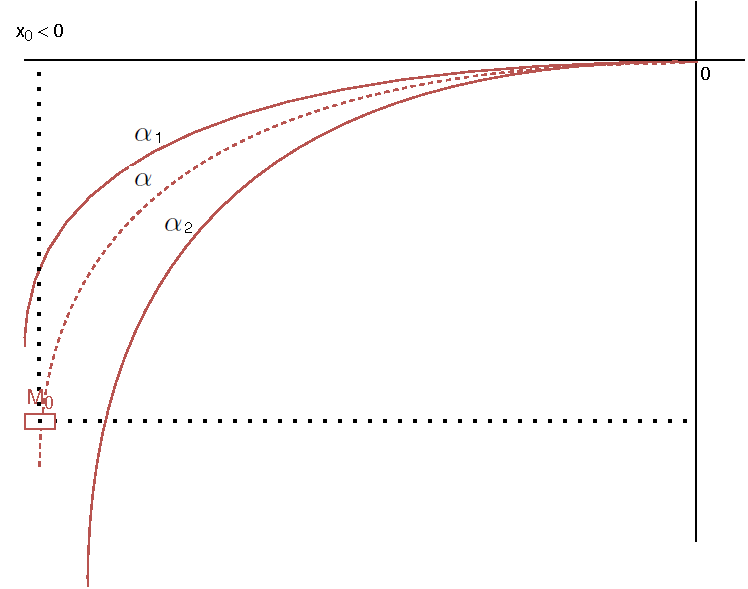
\includegraphics[height=9cm]{images_these/Deux_trajectoires.pdf}}
	\caption[Deux trajectoires. ]{Deux trajectoires $\Gamma_{\alpha1}$ et $\Gamma_{\alpha2}$.}
	\label{Deux_trajectoires}
\end{figure}

\begin{figure}[H]
	\centerline{
		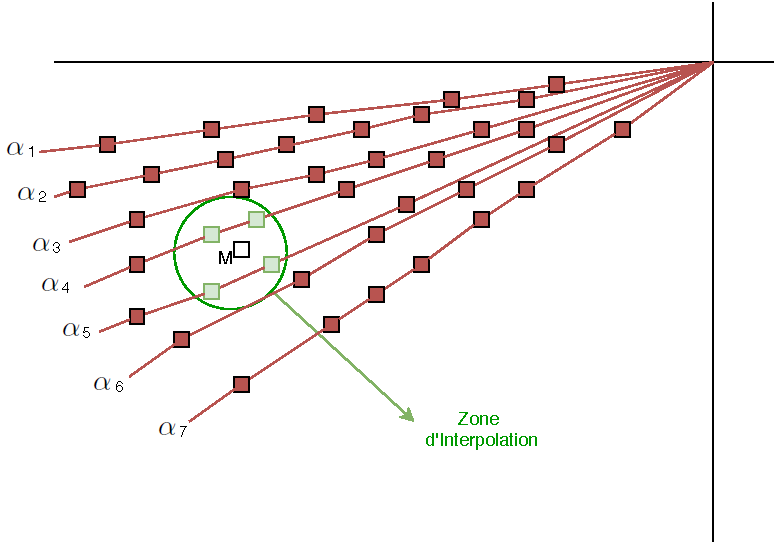
\includegraphics[height=9cm]{images_these/Interpolation.pdf}}
	\caption[Interpolation à partir d'un faisceau de trajectoires. ]{Interpolation à partir d'un faisceau de trajectoires $\Gamma_{\alpha}$.}
	\label{Interpolation}
\end{figure}
}
\poubelle{\subsection{Un Exemple Atypique : Un Jeu de Poursuite}
\label{Jeu_de_Poursuit}
Il arrive que les espaces d'états et de temps d'un schéma \textbf{PD} soient moins naturel que ce qu'on a pu voir jusqu'à présent. Prenons par exemple la situation suivante, dite du \textit{\textbf{Jeu de Poursuite Discret}} :
\begin{itemize}[label=$\square$]
	\item	On se donne un graphe non orienté $G = (X, A)$ : $X $est l'ensemble des sommets, et $A$ celui des arêtes. On se donne également un nombre entier $K$.
	\item	On décide alors de faire jouer $K$ \textit{policiers} et 1 \textit{voleur} de la façon suivante :
	\begin{itemize}
		\item	Les $K$ \textit{policiers} forment une coalition, chacun sachant à chaque instant où sont les autres et où est le \textit{voleur}.  
		\item	Le \textit{voleur} sait à chaque instant où sont les \textit{policiers}.
		\item	Les \textit{policiers} veulent attraper le \textit{voleur}. Chacun des deux blocs ainsi constitués joue à tour de rôle, une fois le \textit{voleur}, une fois les \textit{policiers} et ainsi de suite. La partie se finit quand on repasse deux fois dans le même état (le \textit{voleur} gagne) ou quand un des \textit{policiers} parvient sur le sommet où se trouve le \textit{voleur} (les \textit{policiers} gagnent). Ce sont les \textit{policiers} qui choisissent les premiers leurs positions initiales, le \textit{voleur} décidant ensuite de se placer à son tour.
	\end{itemize}
\end{itemize}
On veut bien sûr calculer une stratégie optimale pour les différents acteurs de ce jeu. Pour les \textit{policiers}, une position $x$ est un vecteur $x =  (x_1,\dots, x_K)$ à valeurs dans $X$, et pour le \textit{voleur}, une position est un sommet $y$ de $X$. Une stratégie pour les \textit{policiers} est donc une fonction $F^P$ qui, à tout couple $(x, y)$ associe $x' =  (x'_1,\dots, x'_K) = F^P(x, y)$ tel que pour tout $k$, $x'_k$ est égal ou adjacent à $x_k$ (on dira que $x'$ est \textit{voisin} de $x$). Une stratégie pour le \textit{voleur} est donc une fonction $F^V$ qui, à tout couple $(x, y)$ associe $y' =  F^V(x, y)$ tel que $ y'$ est égal ou adjacent (on dira que $y'$ est \textit{voisin} de $y$) à $y$.

On procède ici de façon assez similaire au cas continu, c'est-à-dire 
en partant de la fin. L'\textit{espace-temps} correspond au nombre de \textit{mouvements}, c'est-à-dire d'enchainements ($mouvement-voleur \rightarrow mouvement-policier$) dans une partie jouée de façon optimale par chacun des deux joueurs : plus précisément, l'instant 0 signifie que la partie est finie ; l'instant  $- N$ signifie que les \textit{policiers} sont en mesure d'attraper le \textit{voleur} en au plus $N$ \textit{mouvements}, et que le \textit{voleur} est capable de tenir au moins $N-1$ \textit{mouvements} sans être attrapé. 

L'espace d'états est alors, de façon naturelle, l'ensemble des triplets $(x = (x_1,\dots, x_K), y)$ dans $X^{K+1}$, avec la signification : 
\begin{itemize}[label=$\square$]
	\item	les \textit{policiers} sont en $x$, le \textit{voleur} en $y$ ;
	\item	c'est au \textit{voleur} de jouer. 
\end{itemize}	
	A tout état $e =  (x, y)$, on associe une valeur $V(x, y)$ avec la signification :
	\begin{itemize}[label=$\square$]
	\item	Les \textit{policiers} sont en mesure d'attraper le \textit{voleur} en au plus $V(x, y)$ mouvements ; 
	\item	Le \textit{voleur} est capable de tenir au moins $V(x, y) - 1$  mouvements sans être attrapé. Une décision associée est alors un couple $(d_V, d_P)$ qui a la signification suivante :
	\begin{itemize}
		\item	$d_v$ est le mouvement $y'$ voisin de $y$ effectué par le \textit{voleur} telle que pour tout $x'$ voisin de $x$, on ait : $V(x', y') \geq   V(x, y) - 1$ ;  
		\item	$d_P$ est une fonction qui à tout $y'$ voisin de $y$ associe $x'$ voisin de $x$, de telle sorte que $V(x', y') \leq V(x, y) - 1$.  
	\end{itemize}

\end{itemize}
On implémente alors le \textbf{Principe de Bellman} en construisant successivement, selon un processus Backward, les couches $H(N)$, $N \geq 0$, c'est-à-dire les ensembles d'états suivants :	$H(N) = \{$Etats $e = (x, y)$ tels que $V(x, y) = N$, $N$ étant alors impair$\}$.


Ce processus de construction peut être décrit comme suit :

\textbf{Initialisation }:

\begin{itemize}[label=$\square$]
	\item	$H(0) = \{$Etats $e = (x, y)$ tels qu'il existe $k$ avec $x_k = y \}$ ; Aucune décision n'est associée à un tel état $e$, dont la valeur $V$ est nulle ;
\end{itemize}

\textbf{Boucle Principale} : On suppose que l'on a traité les valeurs $0, 1, \dots, N $; Alors :

\begin{itemize}[label=$\square$]
	\item	$H(N) = \{$ Etats $e = (x, y)$ qui ne sont pas dans $ \cup_{0 \leq n \leq N}  H^P(n)$ et qui sont tels que pour tout $y'$ voisin de $y$, il existe $x'$ voisin de $x$ tel que  $(x', y') \in \cup_{0 \leq n \leq N}  H^P(n)\}$ ; 
	\item	Les décisions $(d_V, d_P)$ viennent alors comme suit : 
	\begin{itemize}
		\item V-décision $d_V=\{$  $mouvement-voleur$ $y \rightarrow y'$, tel que pour tout $x'$ voisin de $x$, $(x', y') \notin \cup_{0 \leq n \leq N-1}  H^P(n)\}$;
		\item	P-décision $d_P =\{$ Fonction $mouvement-policier$  $y' \rightarrow f(y')=x'$ adjacent ou égal à $x$, tel que pour tout $y'$ voisin de $y$, $(x', y') \in \cup_{0 \leq n \leq N}  H^P(n)\}$.
	\end{itemize}
\end{itemize}

Le \textit{voleur} possède une stratégie gagnante si pour tout $x$, il existe $y$ tel que $(x, y)  \notin \cup_N (H (N))$. Les \textit{policiers} ayant choisi leur position initiale $x$, le premier mouvement du \textit{voleur} est alors de se placer sur un tel $y$, à chaque mouvement $x \rightarrow x'$ des \textit{policiers}, il se déplace en $y'$ tel que $(x, y)  \notin \cup_N (H (N))$.

La Figure (\ref{Construction}) ci-dessous montre les différents ensembles $H(N)$, dans le cas $K = 1$.
\begin{itemize}
	\item $H(1) = \{(C, A), (B, A), (F, D), (F, E), (F, G), (H, G)\}$
	\item $H(2) = \{(C, E), (CF, D), (H, E)\}$
	\item $H(3)$ est vide $\Rightarrow$ Le \textit{voleur} doit gagner :
	
	\begin{itemize}[label=$\square$]
		\item	Si Policier se place en $H$ ou $G$ alors \textit{voleur} en $C$ ; 
		\item	Si Policier se place en $F$, $E$ ou $D$ alors \textit{voleur} en $B$ ; 
		\item	Si Policier se place en $A$ ou $C$ alors \textit{voleur} en $H$ ; 
		\item	Si Policier se place en $B$ alors \textit{voleur} en $F$.
	\end{itemize}
\end{itemize}
\begin{figure}[H]
	\centerline{
		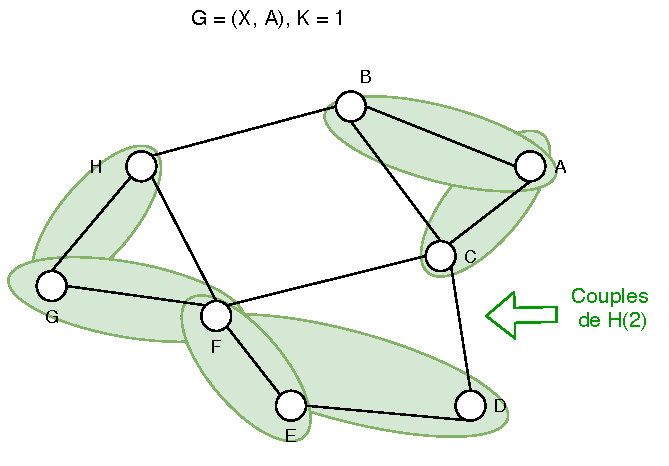
\includegraphics[height=9cm]{images_these/Construction.pdf}}
	\caption[Construction des Ensembles. ]{Construction des Ensembles H(N), avec K = 1.}
	\label{Construction}
\end{figure}

Quoi qu'élégante, et garantissant la polynomialité au sens temps du traitement du Jeu de Poursuite à $K$ \textit{policiers} quand $K$ est fixé, on voit cependant les limites de cette approche : le nombre d'états à manipuler au cours du processus ci-dessus est en $Card(X)^{K+1}$, ce qui dans le cas d'un graphe à 1000 sommets et de cinq \textit{policiers}, va représenter $10^{18}$ états possibles. Si l'on veut être efficace, il faudra alors trouver des procédés de contrôle proches de ceux expliqués en section \ref{Le_Cas_Continu}, et qui tirent partie de la structure du graphe $G$ pour remonter rapidement le long des trajectoires optimales (celles où les deux blocs de joueurs jouent "parfaitement"). 





}\subsection{Le Cas Cyclique}
\label{Le_Cas_Cyclique}

On ne consacrera que peu de place ici à ce dernier cas, malgré son importance pratique. Dans beaucoup de cas, notamment celui des systèmes de gestion de stock et de production, ou bien celui de certains services hospitaliers, on ne peut identifier clairement un début ou une fin. Le système fonctionne selon une certaine forme de périodicité (jour, semaine, mois, année, etc), et il faut organiser au mieux cette périodicité. 

Afin de fixer les idées, on peut reprendre l'exemple initial du système de production, en considérant que la période est de 30 jours (1 mois), numérotés $1,\dots, 30$, avec donc des jours :

$31, 32, \dots, 60, 61, 62, \dots, 90, \dots$ qui reproduisent les demandes $L_i$ enregistrées aux jours $i = 1, \dots, 30$. La question posée est alors simple : Comment définir \textbf{une politique de production/stockage, c'est-à-dire une fonction $d$ qui, à tout instant de base} $i = 1, \dots, 30$, tout état $e = (e_S, e_M)$ associe une décision $d(i, e) = (d_P, d_M)$ appliquée de la même façon à tout instant réel $30\times j + i$, $j = 0, \dots,$ et qui permette :

\begin{itemize}[label=$\square$]
	\item De satisfaire les demandes périodiques $L_i = L_{i+30 \times j}$;
	\item	De minimiser le coût induit par période de 30 jours.
\end{itemize}

Ainsi formulé, notre énoncé laisse apparaitre des zones de flou : 
\begin{itemize}[label=$\square$]
	\item	Par exemple, la notion de périodicité s'applique-t-elle aux états ? En d'autres termes, l'état induit par une trajectoire périodique de notre système à un instant $i$ doit-il être le même pour tous les instants de la forme $30 \times j + i$ ? Ou bien peut-on se contenter de ce que cette périodicité sur les états soit seulement un multiple de 30 ? 
	\item	Egalement, doit-on considérer que l'état courant rencontré quand $i = 1$ (ou 0) fait partie de la \textbf{trajectoire périodique} cherchée, ou bien doit-on considérer qu'il fait partie d'une \textbf{trajectoire transitoire} qui permettra d'atteindre une \textbf{trajectoire stationnaire périodique}? Dans ce dernier cas, doit-on se préoccuper de la durée et du coût de cette trajectoire transitoire ?  
\end{itemize}
On voit que le problème devient dès lors assez vite compliqué, avec la place pour de multiples variantes. Pour simplifier, on va d'abord supposer que :
\begin{itemize}[label=$\square$]
	\item	On exige une périodicité de 30 jours sur les états : pour tout $i$, l'état d'une trajectoire en $i+ 30$ doit être le même que l'état en $i$ ;
	\item	On ne se préoccupe pas de l'état transitoire.
\end{itemize}
Dans ce cas, on voit que l'on cherche un circuit à 30 sommets et de longueur minimale dans un graphe orienté tel que représenté sur la Figure (\ref{Etats_Cycliques}).

\begin{figure}[H]
	\centerline{
		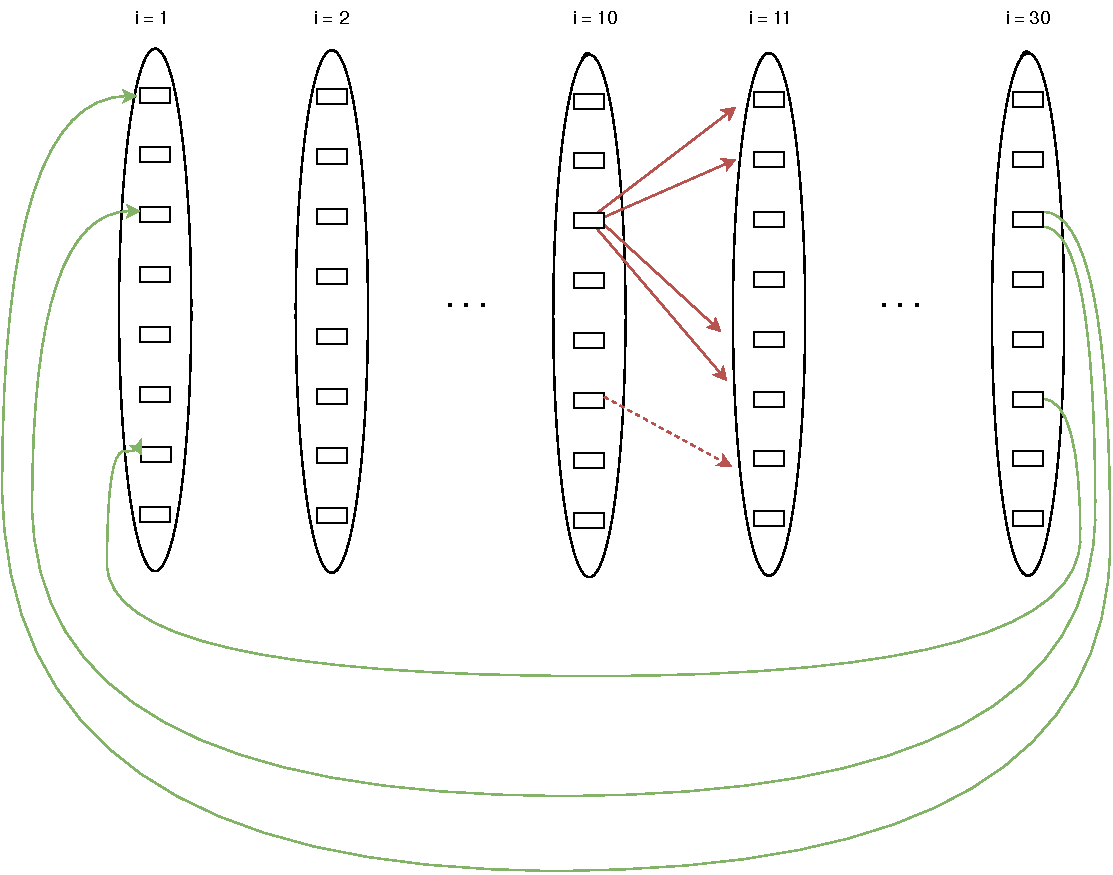
\includegraphics[height=12cm]{images_these/Etats_Cycliques.pdf}}
	\caption[Graphe des Etats Cycliques. ]{Graphe des Etats Cycliques.}
	\label{Etats_Cycliques}
\end{figure}


Une première approche vient comme suit :
\begin{enumerate}
	\item	On applique l'algorithme \textbf{PD}  tel que vu en Section \ref{Cadre_general} à partir de tous les états initiaux $(0, e = (e_S, e_M))$ possibles, en considérant à chaque fois que l'état final est défini comme  $(N+1, e)$. On peut le faire en Backward afin de récupérer plus aisément les suites de décisions pour chaque état. On obtient alors pour chaque état $f$, et chaque $i$, une valeur $V_e(i, f)$
	\item	On choisit e de telle sorte que la valeur $V_e(N+1, e)$ soit minimale. Les séquences de décisions issues de 1) nous fournissent alors notre stratégie.
\end{enumerate}

Sans entrer dans le détail, on voit que cette façon de procéder présente deux inconvénients :

\begin{itemize}[label=$\square$]
	\item	Elle est coûteuse en temps, puisqu'il faut énumérer tous les états e possibles au jour $i = 1$, et leur appliquer le \textbf{PD} de la Section \ref{Cadre_general} ; 
	\item	Elle ne nous dit rien sur les états transitoires, c'est-à-dire ceux par lesquelles il faudra passer avant de stabiliser la trajectoire autour de sa version périodique optimale, alors que dans la pratique, les systèmes réels ne sont jamais vraiment stationnaires.
\end{itemize}

On peut dès lors appliquer une autre approche :
\begin{enumerate}
	\item	On choisit un (ou plusieurs états finaux « plausibles », correspondant au passage en $i = 30 \times j + 1$ ;
	\item	On remonte alors le processus \textbf{PD} vu à la section \ref{Cadre_general}, en stratégie Backward, sur un temps suffisamment long (par exemple de $j = 10 $ jusqu'à $j = 0$) ; 
	\item	On considère alors les décisions correspondant à $j = 0$ comme fournissant les décisions en régime stationnaire ; On répertorie l'ensemble $E_{Stat}$ des états correspondant à $E(0)$ selon le schéma ainsi appliqué ; Pour chaque état $e$ on calcule son coût par période $CP(e)$ ; 
	\item	Pour un état $e_0$ donné à un instant $i = 0$,  on applique le processus \textbf{PD} en Forward à partir de $i = 0$ et $e_0$, en considérant un état final fictif $e_F$ associé à $i = 31$, et une transition fictive permettant de passer de tout couple $(e, 30)$, $e \in E_{Stat}  à (31, e_F)$, et dotée d'un coût $\beta \times CP(e)$, $\beta$ étant un \textit{scaling} coefficient, supposé pondérer les poids respectifs de la partie transitoire et de la partie stationnaire. 
\end{enumerate}

Cette approche suscite aussi des questions et des remarques : 
\begin{itemize}[label=$\square$]
	\item	Comment choisir $\beta$, c'est-à-dire comment équilibrer transitoire et stationnaire ?
	\item	La partie stationnaire de la trajectoire peut ne pas correspondre à 30, mais à un multiple de 30.
\end{itemize}

Dans cette section, nous avons fait un état de l'art de la programmation dynamique. Dans la section suivante, nous présenterons brièvement ce qu'est l'\textit{apprentissage}. 

%\end{itemize}

%	\subsection{Programmation dynamique discrete}
%	\subsection{Programmation dynamique continue (contrôle optimal)}
%	\subsection{Programmation dynamique stochastique}
%	\subsubsection{Programmation dynamique stochastique approchée}
%	\subsubsection{Programmation dynamique duale stochastique}
%	\subsection{Programmation dynamique déterministe}
%	\subsection{Programmation dynamique ittérative}
%	\subsection{Programmation dynamique Probabiliste}
\section{Apprentissage automatique}

L'intelligence artificielle abrégé IA est un concept général qui fait allusion à des systèmes ou machines qui imitent l'intelligence humaine. Le \textit{Machine Learning} abrégé ML est un sous-domaine de l'intelligence artificielle qui apprend et améliore des performances en fonction des données traitées. Le \textit{machine learning } apporte des solutions aux problèmes complexes en analysant de grande quantité de données.
Les principales étapes d'un projet de \textit{machine learning} sont les suivantes : la définition claire du problème à résoudre, l'acquisition des données, la préparation et le nettoyage des données, la séparation des données, le choix des procédés de \textit{machine learning}, l'entrainement des procédés, l'évaluation  et la validation des procédés, le déploiement et la mise en \og production \fg{} des procédés pour résoudre le problème posé.
%\begin{enumerate}
%	\item
%
% La définition claire du problème à résoudre consiste à définir de façon précise la problématique à résoudre afin de mener à bien les étapes suivantes. En effet, si le problème n'est pas bien défini on peut par exemple collecter les mauvaises données ou alors faire un mauvais choix au niveau du choix des procédés à implémenter. 
%	\item
% L'acquisition des données consiste à identifier les différentes sources de données dont on a besoin pour l'entrainement de nos procédés. Il est important de savoir que la qualité de nos procédés dépend fortement des données qu'on utilise. De plus, la quantité de données récoltées influence aussi grandement les performances de nos procédés.
%	\item
% Une autre étape importante est la préparation et le nettoyage des données. Habituellement, les données issus de processus du monde réel ne sont pas structurées, cette étape consiste à structurer ces données. On doit identifier ici les variables (\textit{features}) puis, les diviser en deux catégories à savoir les variables connus et les variables à prédire. On doit identifier le type de chaque variable c'est-à-dire savoir si ce sont des variables catégorielles, discrètes ou continues. On doit corriger les données altérées, inexactes ou non pertinentes pour améliorer leurs cohérences et leurs fiabilités. On doit compléter les valeurs manquantes. On doit s'assurer que les données ne sont pas biaisées, en supprimant par exemple une des variables dupliquées.
%	\item
% Une autre étape est la séparation des données en deux catégories à savoir les données dites \og d'entrainement \fg{} et les données dites de \og test \fg{}. Les données d'entrainement sont utilisées pour entrainer nos procédés et les données de test sont utilisées pour tester les performances des procédés obtenus. Habituellement, on n'utilise pas les données d'entrainement pour tester le procédé car puisqu'elles ont été utilisées pour entrainer le procédé, intuitivement le procédé peut avoir de meilleures performances avec elles. De plus, ce qui nous intéresse c'est de mesurer les performances de nos procédés sur des données qu'il n'a jamais vues, car c'est ce qui se passera dans la réalité. Dans la plus part du temps, on réserve 80 \% des données pour les données d'entrainement et 20 \% pour les données de test. On peut aussi avoir une troisième catégorie de données dites de validation qui permet de choisir entre plusieurs procédés celui qui a les meilleurs performances en fonction des \textit{hyper-paramètres}.
%	\item 
%Une étape cruciale d'un projet de machine learning est le choix des procédés à implémenter et de leurs paramètres. Il existe plusieurs type de procédés à savoir les algorithmes de machine learning supervisés, les algorithmes de machine learning non supervisés et les algorithmes de machine learning semi-supervisés. Un projet de machine learning se termine par 
%	%\item 
%l'entrainement des procédés sélectionnés sur les données dites \og d'entrainement\fg{} et par
%	%\item
%	%\item
%l'évaluation et la validation des procédés sur les données dites de \og test\fg{}.
%\end{enumerate}


%Les procédés en machine learning ont besoin de très grande quantité de données mais il est difficile de manipuler de très grande quantité de données raison pour laquelle un domaine appelé \textit{Big Data} existe.
%Il est difficile de pouvoir identifier le bon type d'outil à utiliser pour pouvoir résoudre un certain type de problématique spécifique en apprentissage. Il faudrait donc bien maitriser les avantages et inconvénients des procédés existants.
%Il est aussi difficile d'identifier ce qui fait qu'un procédé n'est pas performant pour un certain type de problème, es-ce à cause de la qualité (\textit{bruit dans les données}) ou la quantité de données utilisées ? Es-ce à cause des paramètres du procédé ? Car il est difficile d'identifier les bons paramètres et hyper-paramètres de nos procédés à cause du très grand nombre qui existent dans la pratique, il devient donc difficile de tester toutes les combinaisons possibles. Quand bien même des procédés de correction existeraient, ceux-ci sont trop lourd en temps de traitement.
%Enfin, une autre difficulté en apprentissage est le sur-apprentissage qui est cette tendance qu'à un procédé à faire de bonnes prédictions uniquement sur les données d'entrainement et à faire de mauvaises prédictions sur de nouvelles données.

Dans cette section, nous commencerons par identifier les principales difficultés de l'apprentissage. Nous nous attarderons ensuite sur les réseaux de neurones car nous avons utilisé cette technique pour faire une approximation des coûts de notre problème. Nous finirons par présenter l'API Keras de Tensorflow Keras utilisé pour implémenter nos réseaux de neurones.

\subsection{La problématique générale de l'apprentissage}


La problématique de l'apprentissage est confrontée à plusieurs difficultés que nous présentons dans cette section.
La problématique de l'apprentissage est dans la plupart des cas une
problématique d'approximation. C'est une correspondance $R$ qui à une entrée $I$
associe une sortie complexe $O$, que l'on veut approcher via un procédé $I  \rightarrow A^\lambda(I)$,
où $\lambda$est le jeu de paramètres à apprendre, et où $A^\lambda$ est un algorithme
rapide. Le but est que l'erreur commise en remplaçant O par $A^\lambda(I)$ soit faible. Cette erreur
pouvant être mesurée :
\begin{itemize}[label=$\square$]
\item Comme pourcentage de fois où $O$ et $A^\lambda(I)$ sont différents, dans le cas ou
$O$ désigne un identificateur de classe ou bien une propriété ;
\item Comme une valeur moyenne
de $(A^\lambda(I)- O)$ dans le cas où $O$ désigne une quantité ou un vecteur de nombres. 
\end{itemize}
Ce dernier point est
notamment le cas pour ce qui est de notre étude, puisque l'on veut remplacer un algorithme
complexe de programmation dynamique par un algorithme plus simple que l'on puisse utiliser
comme estimateur de solution au sein d'un processus d'optimisation.

Les points durs de la mise en œuvre d'un projet d'apprentissage sont les
suivants : le premier point est l'identification de la correspondance $I \rightarrow O$ que l'on veut soumettre
à apprentissage, le deuxième point dur porte sur le choix du type de procédé $A^\lambda$ dont on va se servir et le troisième point dur porte sur l'obtention de données.
%\begin{itemize}[label=$\square$]
	%\item
	
	Afin d'illustrer la difficulté d'identifier la correspondance $I \rightarrow O$ que l'on veut soumettre
	 à apprentissage, on peut se référer au jeu des échecs : on
	veut utiliser l'apprentissage afin de construire un logiciel qui joue bien, et donc, qui, face
	à une position $P$ donnée (un état de l'échiquier) choisisse le bon mouvement $M$ à
	effectuer. Que faut-il alors chercher à apprendre : la correspondance $P \rightarrow 
	M$, ou bien une correspondance auxiliaire $P \rightarrow Qualite(P)$ qui nous fournit une estimation
	de la qualité du jeu du point de vue du joueur machine ? L'expérience montre que seule
	la deuxième approche permettra d'obtenir de bons résultats.
	%\item 
	
	Le procédé $A^\lambda$ dont on va se servir peut être une formule portant sur des indicateurs caractéristique de $I$ ; il peut aussi être un système à base de règles (systèmes expert) ; il peut enfin être un automate
	relativement complexe tel qu'un réseau neuronal ou bien un automate SVM.
	%\item
	
	 L'obtention de données, c'est-à-dire de couples $(I, O)$, où
	$I$ est une instance et $O$ un résultat théorique associé à I, est une tâche complexe. Il faut que l'on dispose de
	nettement plus de tels couples $(I, O)$ que de paramètres $\lambda$ à apprendre, et il faut veiller à
	ce que ces instances $I$ soient suffisamment diversifiées. Ceci peut s'avérer difficile et pose la question de l'apprentissage
	supervisé : dans le cas supervisé, on dispose de suffisamment de coule $(I, O)$
	d'entrainement, et on ajuste le vecteur de paramètres $\lambda$grâce à ces instances ; dans le
	cas contraire, il faut faire en sorte que le procédé $A^\lambda$ apprenne lui-même le vecteur $\lambda$, en
	corrigeant de lui-même ses erreurs. On parle alors d'apprentissage non supervisé : autoapprentissage,
	apprentissage par renforcement,etc . Mettre en oeuvre un procédé
	d'apprentissage non supervisé est dans tous les cas quelque chose de difficile.
%\end{itemize}

%\subsection{L'apprentissage supervisée et l'apprentissage non-supervisée}
%Pour faire de l'apprentissage supervisé, on a besoin d'un ensemble de données étiquetés. Une étiquette d'une donnée est une classe à laquelle appartient cette donnée. On veut pouvoir prédire à quelle classe appartient une donnée quelconque. Lorsque la valeur prédite est une classe, on appelle ce type de procédé un procédé de classification. Mais lorsque la valeur prédite est une valeur numérique, on appelle ce type de procédés un procédé de régression.
 

%Pour faire de l'apprentissage non-supervisé, on a besoin d'un ensemble de données qui n'ont pas d'étiquettes. Dans ce type d'apprentissage on ne connait pas le nombre de classes que forme les données, et on cherche à le calculer puis, à prédire à quelle classe appartient une donnée quelconque. Par exemple, le clustering fait partie de ce type d'apprentissage.

%Il existe une troisième catégorie d'algorithmes en machine learning appelée algorithme de machine learning semi-supervisé. Ici on entraine nos procédés simultanément avec des données étiquetées et des données non étiquetées.
\subsection{Les réseaux de neurones artificiels}

Les réseaux de neurones artificiels cherche à simuler le comportement des neurones du cerveau humain \cite{mcculloch43a}. Ce sont des intelligences artificielles qui donnent aux ordinateurs la capacité d' \og apprendre à apprendre \fg{} et par la suite, à agir et réagir comme les humains, en améliorant leur mode d'apprentissage et leurs connaissances de façon autonome sur la durée. Les réseaux de neurones ont une pléthore d'applications parmi lesquelles ont peut citer : le traitement d'images (la reconnaissance faciale, la détection d'objets), le traitement de la langue et le traitement du signal.
\subsubsection{Description générale et représentation graphique d'un réseau de neurones}
Un réseau de neurones est généralement représenté comme une succession de \og couches \fg{}. Chaque couche contient 1 ou plusieurs neurones. Les neurones d'une couche sont reliés aux neurones de la couche suivante de manière complète, voir figure (\ref{RN_all_connect}), ou partielle, voir figure (\ref{RN_partial_connect}).

\begin{figure}[H]
	\centerline{
		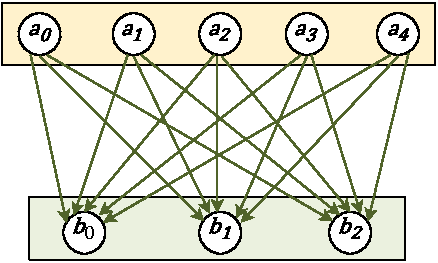
\includegraphics[height=5cm]{images_these/RN_all_connect.pdf}}
	\caption[Une couche de 5 neurones complétement reliée à une couche de 3 neurones. ]{Représentation d'une couche de 5 neurones \textbf{complétement} reliée à une couche de 3 neurones.}
	\label{RN_all_connect}
\end{figure}

\begin{figure}[H]
	\centerline{
		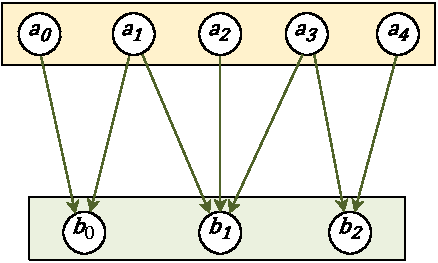
\includegraphics[height=5cm]{images_these/RN_partial_connect.pdf}}
	\caption[Une couche de 5 neurones partiellement reliée à une couche de 3 neurones. ]{Représentation d'une couche de 5 neurones \textbf{partiellement} reliée à une couche de 3 neurones.}
	\label{RN_partial_connect}
\end{figure}

Chaque neurone $j$ a une valeur d'entrée $in(j)$ (aussi appelée valeur de préactivation) et une valeur de sortie $out(j)$ (aussi appelée valeur d'activation). Dans le cas où la fonction d'agrégation est la somme pondéré, la valeur d'entrée d'un neurone est égale à la somme des valeurs de sortie des neurones le précédant, pondérée par des poids, à laquelle on ajoute un biais. Les poids sont souvent représentés sur les arcs et le biais est souvent représenté comme un neurone supplémentaire, de valeur de sortie 1 (fixe) avec un poids $B$, voir figure (\ref{RN_poids_biais}). La valeur de sortie d'un neurone est égale à sa valeur d'entrée à laquelle on applique une fonction dite d'activation. La figure (\ref{RN_in_outt}) donne les valeurs d'entrée et de sortie du neurone $b$ de la figure (\ref{RN_poids_biais}) avec une fonction d'activation $\phi$.

\begin{figure}[H]
	\centerline{
		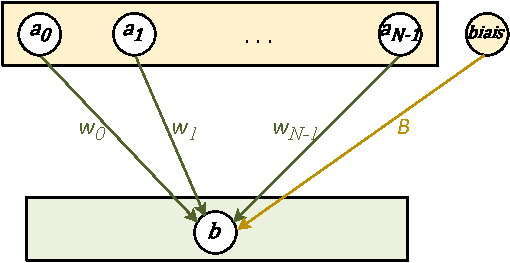
\includegraphics[height=5cm]{images_these/RN_poids_biais.pdf}}
	\caption[Représentation des poids et du biais. ]{Représentation des poids et du biais.}
	\label{RN_poids_biais}
\end{figure}

\begin{figure}[H]
	\centerline{
		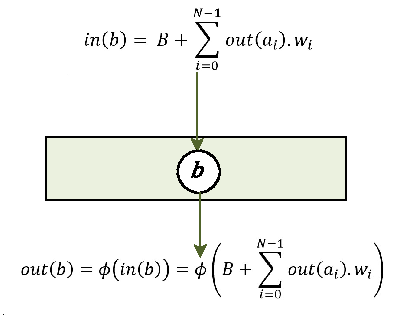
\includegraphics[height=6cm]{images_these/RN_in_outt.pdf}}
	\caption[Calcul des valeurs d'entrée et de sortie d'un neurone. ]{Calcul des valeurs d'entrée et de sortie du neurone $b$ du réseau de la Figure (\ref{RN_poids_biais}).}
	\label{RN_in_outt}
\end{figure}
Il existe plusieurs types de fonction d'activation parmi lesquelles on peut citer : 
\begin{itemize}[label=$\square$]
	\item La fonction linéaire :
	$f(x)=x$
	\item La fonction sigmoïde : 
	${\displaystyle f(x)={\frac {1}{1+{\rm {e}}^{-x}}}}$
	\item La fonction RELU :
	$$
	f(x)= \left\{
	\begin{array}{ll}
	0 & \mbox{si x<0} \\
	x & \mbox{si x $\geq$ 0.}
	\end{array}
	\right.
	$$
	\item La fonction softmax :
	${\displaystyle f(x)_j={\frac {e^{x_j}}{\sum_{k=1, \dots K}e^{x_k}}}$ pour tout $j \in \{1, \dots, K\}$, dans ce cas $\sum_j f(x)_j=1$.
	\end{itemize}

Dans le cas général, il y a plusieurs neurones par couche et les poids utilisés pour calculer la valeur d'entrée d'un neurone sont différents d'un neurone à l'autre, ainsi que les biais, voir Figure (\ref{RN_poids_biais--}). On a pour habitude de regrouper ces poids dans une matrice, voir Figure (\ref{RN_matrice_poids}).
\begin{figure}[H]
	\centerline{
		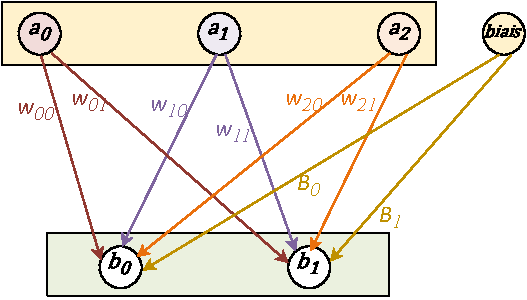
\includegraphics[height=6cm]{images_these/RN_poids_biais--.pdf}}
	\caption[Poids et biais entre deux couches de neurones non unitaires. ]{Poids et biais entre deux couches de neurones non unitaires.}
	\label{RN_poids_biais--}
\end{figure}

\begin{figure}[H]
	\centerline{
		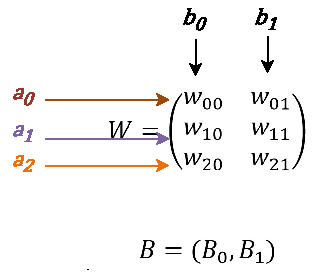
\includegraphics[height=6cm]{images_these/RN_matrice_poids.pdf}}
	\caption[Une matrice des poids $W$ et un vecteur des biais $B$. ]{Matrice des poids $W$ et vecteur des biais $B$ associés à la Figure (\ref{RN_poids_biais--}).}
	\label{RN_matrice_poids}
\end{figure}
 %le vecteur $O$ des impulsions de sorties, qui représente la caractéristique de comportement que l'on veut estimer : identificateur d'une classe d'appartenance pour un objectif de classification,propriété en $\{0, 1\}$ pour un objectif de reconnaissance de forme,valeur réelle, identifiant une qualité, une performance,etc.


\subsubsection{Description du fonctionnement des réseaux de neurones}

Le fonctionnement général du processus d'apprentissage est :
\begin{itemize}[label=$\square$]
	\item Pour une entrée $I$, on calcule l'objet de sotie $A^\lambda(I) = O^\lambda$, calculée par le réseau $A^\lambda$ ($\lambda$ désigne le vecteur de coefficients synaptique et de biais à apprendre) ; Puis on évalue l'erreur $Err(O^\lambda)$ induite par rapport à un résultat souhaité ; Puis on ajuste $\lambda$ afin de diminuer cette erreur en appliquant une formule $\lambda \leftarrow  \lambda - \delta.Grad(Err(O^\lambda))$, où $\delta$ est une petite valeur positive, qu'on nomme le pas.
	\item On applique ce processus pour un ensemble d'instances $I$ (ou de paquets d'instances) dites d'entrainement, générées aléatoirement. Le processus global ainsi induit est dit de \textbf{Gradient Stochastique}. C'est parce que l'on a besoin de pouvoir calculer cette quantité gradient $Grad(Err(O^\lambda))$ que l'on utilise des coefficients synaptiques et des impulsions continues, ainsi que des fonctions d'activation différentiables.
\end{itemize}

\subsubsection{Difficultés liées à la mise en œuvre de réseau de neurones}

Les difficultés liées à la mise en œuvre des réseaux de neurones sont :
\begin{itemize}[label=$\square$]
	\item Une première difficulté tient à la conception du réseau : il n'existe à ce propos pas de méthode clairement reconnue. L'intuition est toutefois d'essayer d'épouser la logique du fonctionnement de la correspondance $I \rightarrow O$ que l'on cherche à apprendre.
	\item Une deuxième difficulté majeure tient au fait qu'un réseau neuronal tend à mettre en jeu un nombre important de coefficients à apprendre, ce qui signifie qu'il faut aussi un nombre important d'instances $I$ pour les phases d'entrainement et de validation (à priori sensiblement plus que de coefficients synaptiques). Obtenir ces instances en même temps que leur résultat souhaité $O$ peut constituer une vraie difficulté. Si le nombre d'instances est insuffisant, alors on risque de bien réussir la phase entrainement, mais d'avoir un échec sur la phase validation. Une difficulté en apprentissage est le sur-apprentissage qui est cette tendance qu'à un procédé à faire de bonnes prédictions uniquement sur les données d'entrainement et à faire de mauvaises prédictions sur de nouvelles données.
	
\end{itemize}

\subsection{L'API Keras de Tensorflow Keras}

Dans cette section, on note Tensorflow Keras de manière abrégée : tf.keras. De plus, nous utiliserons le vocabulaire suivant :

\begin{itemize}[label=$\square$]

	\item 	le terme \textbf{couche} sera utilisé pour la description générale d'un réseau alors que le terme \textbf{layer} sera utilisé pour faire référence à une couche particulière prédéfinie de tf.keras ;
	\item 	les termes \textbf{modèle} et \textbf{réseau} seront utilisés indistinctement (modèle étant le vocabulaire utilisé dans tf.keras pour faire référence à un réseau de neurones).
\end{itemize}

\subsubsection{Les couches et les poids dans tf.keras}
\label{couche_poids_tfkeras}
Dans tf.keras il existe différentes couches, appelées layers, que l'on peut utiliser facilement pour créer un réseau de neurones (également appelé modèle). Ces layers définissent la manière dont les neurones reçoivent l'information des layers précédents. 
\begin{itemize}[label=$\square$]
\item \textbf{Le layer Dense}

Le layer Dense est le layer de référence pour créer des couches dont les neurones reçoivent en entrée une valeur égale à la somme pondérée de l'ensemble des neurones du layer précédent (comme dans la Figure (\ref{RN_poids_biais--})). Le layer Dense permet donc de créer une couche qui est reliée de manière complète à la couche précédente. 
Le code suivant montre comment créer le réseau de la Figure (\ref{RN_poids_biais--}).
\begin{lstlisting}
#création de la couche des inputs (avec 3 neurones, car les entrées sont de taille 3)
my_input = keras.Input(shape=(3,), name="input") 

# création de la couche de sortie avec 2 neurones
sortie = keras.layers.Dense(2, activation='linear', name="sortie")(my_input)

#construction du modèle
model = keras.Model(inputs=my_input, outputs=sortie)

\end{lstlisting}
Dans tf.keras, les couches sont représentées par une matrice des poids et un vecteur des biais. 
La fonction suivante permet d'afficher les poids d'une couche. Elle prend en paramètre le modèle et le nom de la couche dont on souhaite afficher les poids.
\begin{lstlisting}
def affichePoids(model, name):

	print ("affichage des poids de la couche", name)

	#afficher les poids qui arrivent  sur une couche
	WS = model.get_layer(name).get_weights()

	print("weights = ", WS[0] )
	print("biais = ", WS[1] )

\end{lstlisting}
Par exemple, si on souhaite afficher les poids de la couche de sortie du modèle Dense précedent il faut écrire affichePoids(model, "sortie"). Les poids sont alors affichés comme à la figure (\ref{RN_exemple_poids}). La représenttion graphique de ces poids est à la figure (\ref{RN_exemple}).
\begin{figure}[H]
	\centerline{
		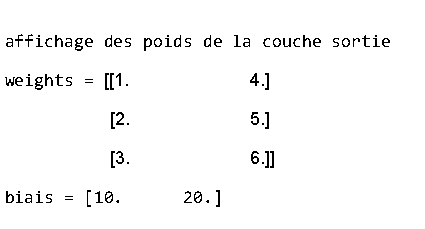
\includegraphics[height=4cm]{images_these/RN_exemple_poids.pdf}}
	\caption[Affichage des poids.]{Affichage des poids.}
	\label{RN_exemple_poids}
\end{figure}
\begin{figure}[H]
	\centerline{
		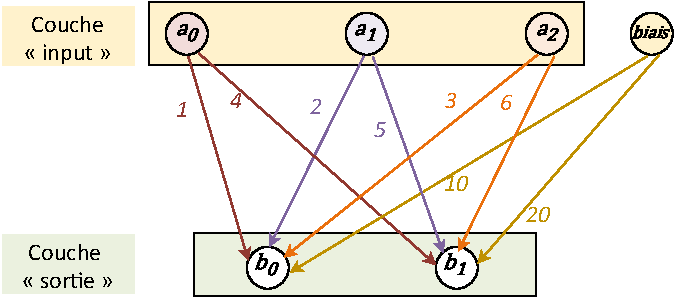
\includegraphics[height=6cm]{images_these/RN_exemple.pdf}}
	\caption[Représentation graphique des poids associés à la Figure (\ref{RN_exemple_poids}). ]{Représentation graphique des poids associés à la Figure (\ref{RN_exemple_poids}).}
	\label{RN_exemple}
\end{figure}
Ils signifient que les valeurs d'entrée (ou de préactivation) pour les 2 neurones $(b_0, b_1)$ de la couche de sortie sont calculées de la manière suivante (pour simplifier les notations \textit{out}$(a)$ est remplacé par $a$) :
\textit{in}$(b_0)=a_0+2a_1+3a_2+10$, \textit{in}$(b_1)=4a_0+5a_1+6a_2+20$.

\item \textbf{Initialisation des poids du layer Dense}

L'initialisation des poids est un élément important qui joue un rôle clé dans la descente du gradient. Par défaut cette initialisation est réalisée par tf.keras de manière aléatoire. Cependant, si on a une idée des poids finaux, il peut être intéressant de réaliser cette initialisation nous-même. Il suffit pour cela de passer en paramètre la matrice des poids et le vecteur des biais lors de la création du layer Dense.
Le code suivant montre comment construire le réseau de la Figure (\ref{RN_exemple}) en initialisant les poids (y compris les biais) à la main.

\begin{lstlisting}
# création de la couche des inputs (avec 3 neurones)
my_input = keras.Input(shape=(3,), name="input") 

# création de la couche de sortie avec un 2 neurones et initialisation des poids
my_biais = np.array([10, 20])
my_poids = np.array([[1, 4], [2, 5], [3, 6]])
sortie = keras.layers.Dense(2, activation='linear', weights=[my_poids, my_biais], name="sortie")(my_input)

# construction du modèle
model = keras.Model(inputs=my_input, outputs=sortie)

# dessin du modele
keras.utils.plot_model(model, "Func_tutoPoids2.png", show_shapes=True, dpi=192)
\end{lstlisting}

\item \textbf{Différentes manières de fusionner les couches : \textit{Merging layers}}

tf.keras offre la possibilité de fusionner, de différentes manières, une ou plusieurs couches d'un réseau. Pour cela il faut utiliser des layers particuliers appelés merging layers. 

\begin{itemize}
\item	\textbf{Concaténation de plusieurs couches}

La manière la plus simple de fusionner des couches est de les concaténer : dans ce cas les neurones sont simplement recopiés de leur couche initiale vers la couche de concaténation sans modification de leur valeur de sortie.
Le code suivant montre comment concaténer 3 couches à l'aide du layer \textit{Concatenate}. 
%La représentation graphique de cela est la figure (\ref{concat}).
\begin{lstlisting}
# création de 3 couches des entrées de taille respective 3, 2 et 4
my_input1 = keras.Input(shape=(3,), name="input1") 
my_input2 = keras.Input(shape=(2,), name="input2") 
my_input3 = keras.Input(shape=(4,), name="input3") 

# concaténation des 3 couches des entrées 
concat = keras.layers.concatenate([my_input1, my_input2, my_input3])

# création de la couche de sortie avec un 2 neurones
sortie = keras.layers.Dense(2, activation='linear', name="sortie")(concat)

# construction du modèle
model = keras.Model(inputs=[my_input1, my_input2, my_input3], outputs=sortie)
\end{lstlisting}

%\begin{figure}[!ht]
%	\centerline{
%		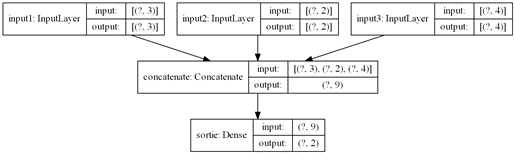
\includegraphics[height=6cm]{images_these/concat.png}}
%	\caption[Concaténation de 3 couches. ]{Concaténation de 3 couches à l'aide du layer \textit{Concatenate}.}
%	\label{concat}
%\end{figure}

\item	\textbf{Multiplication terme à terme de deux couches}

Un autre layer très intéressant est le layer Multiply. Il permet de multiplier la valeur de sortie de 2 couches de neurones terme à terme. L'extrait de code suivant illustre son utilisation.

\begin{lstlisting}
# création de 2 couches d'entrée de taille 3
my_input1 = keras.Input(shape=(3,), name="input1") 
my_input2 = keras.Input(shape=(3,), name="input2") 

# une couche cachée par couche d'entrée
couche1 = keras.layers.Dense(3, activation='relu', name="C1")(my_input1)
couche2 = keras.layers.Dense(3, activation='relu', name="C2")(my_input2)

# multiplication des 2 couches précédentes 
sortie = keras.layers.Multiply()([couche1, couche2])
\end{lstlisting}
\item \textbf{Afficher la sortie des couches internes d'un modèle}

Afin de s'assurer que les couches ont été fusionnées comme on l'entend, nous avons besoin d'accéder à la sortie des couches internes d'un modèle. Pour cela il faut : 
\begin{enumerate}
\item	Récupérer la couche du modèle concernée à l'aide de son nom (il faut donc lui avoir donné un nom lors de sa création),
\item	Appeler la couche avec les inputs du modèle pour lesquels on souhaite connaître la sortie.
\end{enumerate}
Le code suivant illustre ceci sur le modèle précédenmment créé.

\begin{lstlisting}
# exemple de données pour les 2 couches input
in1_test = np.asarray([[1,2,3]])
in2_test = np.asarray([[4,5,6]])

# on recupère les couches internes à partir de leur nom
c1_layer = keras.Model(inputs=model.input, outputs=model.get_layer('C1').output)
c2_layer = keras.Model(inputs=model.input, outputs=model.get_layer('C2').output)

# on donne aux couches internes les inputs souhaités
couche1_out = c1_layer({'input1' : in1_test, 'input2':  in2_test})
couche2_out = c2_layer({'input1' : in1_test, 'input2':  in2_test})

# on recupère la sortie du modèle avec les inputs souhaités
sortie_out = model.predict({'input1' : in1_test, 'input2':  in2_test})

# on affiche la sortie des différentes couches 
print('couche1 : ', couche1_out)
print('couche2 : ', couche2_out)
print('sortie : ', sortie_out)
\end{lstlisting}

On obtient, par exemple, l'affichage suivant :

couche1 : tf.Tensor([[-1.399934  -2.0355947  3.6685464]], shape=(1, 3), dtype=float32)

couche2 : tf.Tensor([[0.         4.4896154  0.15367174]], shape=(1, 3), dtype=float32)

sortie : [[-0.         -9.139037    0.56375194]]

On constate que la couche de sortie est bien la multiplication terme à terme des couches internes 1 et 2.

\textbf{NB}. Si vous testez ce code vous n'obtiendrez probablement pas la même chose, les poids étant initialisés de manière aléatoire.

\end{itemize}
\end{itemize}

\subsubsection{Relier deux couches de neurones de manière partielle}
\begin{itemize}[label=$\square$]
\item \textbf{Problématique générale}

Il n'existe pas, à notre connaissance, de layer prédéfini qui permette de relier 2 couches de manière partielle (c'est-à-dire telle que présentée dans la Figure (\ref{RN_partial_connect})). 

Une solution possible serait de créer son propre layer (ce qui est réalisable dans tf.keras en créant une classe dérivée de la classe Layer). Cependant cette technique demande une très bonne compréhension des différents éléments qui forment un layer au sens de tf.keras ainsi que de la manière dont ils s'articulent. Elle semble, par conséquent, assez fastidieuse à mettre en place.

Une autre solution, qui est celle que nous avons choisis de présenter ici, consiste à utiliser les layers de tf.keras prédéfinis et à les combiner de manière à obtenir exactement la topologie de réseau souhaitée. C'est l'objet de la prochaine sous-section. 

\item \textbf{Combiner des layers prédéfinis de tf.keras pour relier 2 couches de manière partielle}
\begin{Rem}
	Dans cette section, on ne s'intéresse qu'aux arcs (et donc qu'aux poids) entre 2 couches de neurones. Le biais n'est pas pris en compte, et, même s'il existe, on ne le représente pas sur les schémas afin de ne pas surcharger les illustrations. 
\end{Rem}
\begin{itemize}
\item	\textbf{Principe général}

L'idée générale est la suivante : supposons que l'on souhaite créer une couche A de N neurones $(a_0, \dots ,a_{N-1})$ qui envoie de l'information à une couche B de M neurones $(b_0, \dots ,b_{M-1})$. De plus nous souhaitons choisir exactement quel neurone de la couche A envoie de l'information à quel neurone de la couche B (Figure (\ref{RN_2_couches_partielles})). Nous avons donc besoin de pouvoir manipuler chaque neurone de manière indépendante. Nous réalisons cela en 4 étapes (voir (Figure (\ref{Dense_et_Concatenate})) :

\begin{figure}[H]
	\centerline{
		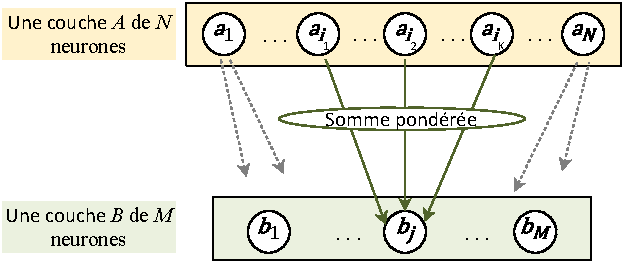
\includegraphics[height=5cm]{images_these/RN_2_couches_partielles.pdf}}
	\caption[Représentation d'un réseau avec 2 couches partiellement reliées.]{Représentation d'un réseau avec 2 couches partiellement reliées.}
	\label{RN_2_couches_partielles}
\end{figure}

\begin{figure}[H]
	\centerline{
		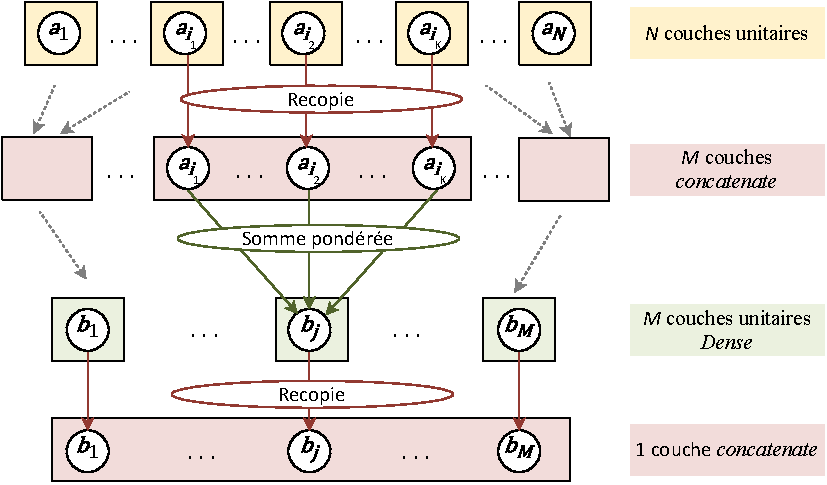
\includegraphics[height=7cm]{images_these/RN_Dense_et_Concatenate.pdf}}
	\caption[Représentation du réseau de la figure (\ref{RN_2_couches_partielles}) en utilisant exclusivement des layers tf.keras Dense et Concatenate.]{Représentation du réseau de la figure (\ref{RN_2_couches_partielles}) en utilisant exclusivement des layers tf.keras Dense et Concatenate.}
	\label{Dense_et_Concatenate}
\end{figure}
\begin{enumerate}
\item	Créer N « sous-couches » unitaires $A_0,\dots,A_{N-1}$ au lieu d'une couche de N neurones : la sous-couche $A_{i,(i=0 \dots N-1)}$ contient uniquement le neurone $a_i$.
	
\item Pour chaque neurone $b_{j,(j=0 \dots M-1)}$ de la couche $B$, identifier les neurones $a_{i_1 },\dots,a_{i_K}  (0\leq i_1\leq i_K \leq N-1)$ qui envoient de l'information à $b_j$. Concaténer les sous-couches $A_{i_1 }, \dots, A_{i_K }$ correspondantes. On obtient ainsi $M$ nouvelles sous-couches $C_0, \dots, C_{M-1}$ de type Concatenate. Notons qu'un même neurone $a_{i, (i=0 \dots N-1)}$  peut se retrouver dans plusieurs sous-couches Concatenate (sa valeur sera la même dans toutes les sous-couches).

\item Créer $M$ sous-couches unitaires $(B_0,\dots,B_{M-1})$ telles qu'une sous-couche $B_{j, (j=0 \dots M-1)}$ contient uniquement le neurone $b_j$ et reçoit en entrée la sortie de la sous-couche $C_j$. 

\item Pour finir, concaténer les sous-couches unitaires $(B_0,\dots,B_{M-1})$ de sorte de retrouver une couche de M neurones $(b_0, \dots, b_{M-1})$.

\end{enumerate}
\begin{Rem}
	Les entiers N et M peuvent être potentiellement grands et/ou inconnus au moment où on écrit le code (par exemple si on les lit dans un fichier). C'est pourquoi il semble judicieux d'utiliser des tableaux pour stocker les différentes sous-couches. 
\end{Rem}

La sous-section suivante illustre ceci sur un exemple.

\item 	\textbf{Illustration sur un exemple}

On souhaite représenter le réseau de la Figure (\ref{RN_partial_connect}) en utilisant uniquement des layers Dense et Concatenate et en suivant la méthodologie donnée en section 3.2.1.

Le résultat obtenu est représenté Figure (\ref{RN_pc_Dense_Concatenate}).


\begin{figure}[H]
	\centerline{
		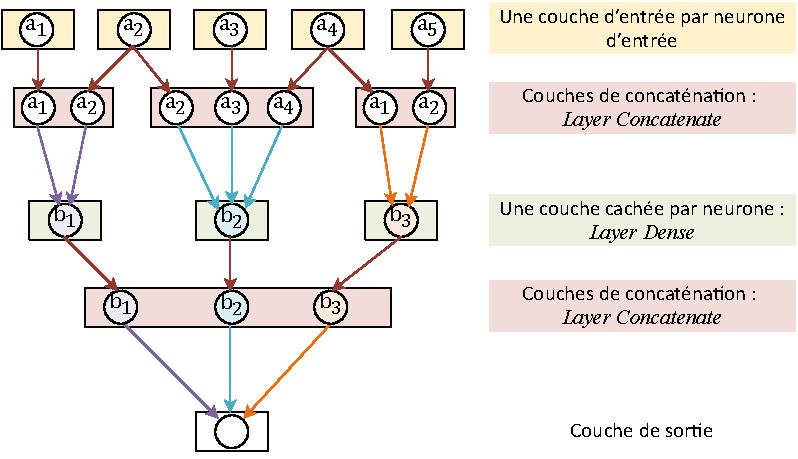
\includegraphics[height=7cm]{images_these/RN_pc_Dense_Concatenate.pdf}}
	\caption[Le réseau de la figure (\ref{RN_partial_connect}) représenté avec des layers Dense et Concatenate.]{Le réseau de la figure (\ref{RN_partial_connect}) représenté avec des layers Dense et Concatenate.}
	\label{RN_pc_Dense_Concatenate}
\end{figure}
Le code qui permet de programmer ce réseau est donné ci-dessous.

\begin{lstlisting}
# ETAPE 2.1 : création des sous-couches A_0 ... A_{N-1} (ici N = 5)

N = 5
ssCoucheA = []

for i in range(N):
tmp = keras.Input(shape=(1,), name="input"+str(i)) 
ssCoucheA.append(tmp)

# ETAPE 2.2 : on crée les M = 3 couches de concaténation 

ssCoucheC = []

ssCoucheC.append(keras.layers.concatenate([ssCoucheA[0], ssCoucheA[1]]))
ssCoucheC.append(keras.layers.concatenate([ssCoucheA[1], ssCoucheA[2], ssCoucheA[3]]))
ssCoucheC.append(keras.layers.concatenate([ssCoucheA[3], ssCoucheA[4]]))


# ETAPE 2.3 :  création des sous-couches B_0 ... B_{M-1} (ici M = 3)
ssCoucheB = []
M = len(ssCoucheC)
for i in range(M):
ssCoucheB.append(keras.layers.Dense(1, activation='linear')(ssCoucheC[i]))

# ETAPE 2.4 :  on concatene les sous-couches B
sortie = keras.layers.concatenate(ssCoucheB)

# construction du modèle : définition des couches d'entrée et de sortie
model = keras.Model(inputs=ssCoucheA, outputs=sortie)

# dessin du modele
keras.utils.plot_model(model, "reseauFunctionalSparse.png", show_shapes=True, dpi=192)

\end{lstlisting}

\end{itemize}
\end{itemize}

\subsubsection{Fixer des poids dépendant des instances}
Le but de cette section est de montrer comment on peut prendre en compte, à l'intérieur d'un réseau, et de manière explicite, des valeurs propres à chaque instance. 
Pour fixer les idées, nous allons illustrer notre propos sur le réseau de la 
Figure (\ref{RN_poids_fixes}). Dans cet exemple nous supposons qu'une entrée est formée de deux types de valeurs : 
N valeurs $a_0, a_1, \dots, a_{N-1}$  
M coefficients $\lambda_0,\lambda_1, \dots ,\lambda_{M-1}$

Les valeurs $a_0, a_1, \dots, a_{N-1}$  sont les entrées du réseau alors que les coefficients $\lambda_0,\lambda_1, \dots,\lambda_{M-1}$ sont utilisés uniquement pour calculer la valeur de sortie du réseau $s$ qui est telle que :
\begin{center}
$s=\sum_{j=0}^{M-1} \lambda_j \times out(b_j)$
\end{center}
où $b_{j,(j=0, \dots, M-1)}$ est le $j^{eme}$  neurone de la couche précédant la sortie du réseau (voir 
Figure (\ref{RN_poids_fixes}))

\begin{figure}[H]
	\centerline{
		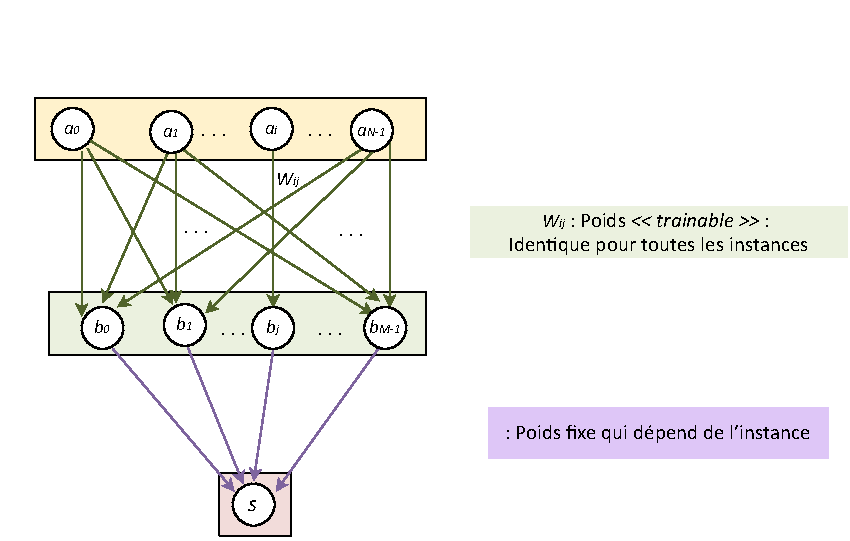
\includegraphics[height=8cm]{images_these/RN_poids_fixes.pdf}}
	\caption[Exemple de réseau dans lequel des poids fixes et dépendant de l'instance interviennent.]{Exemple de réseau dans lequel des poids fixes et dépendant de l'instance interviennent.}
	\label{RN_poids_fixes}
\end{figure}
Nous avons vu dans comment fixer les poids d'un layer Dense. Malheureusement, cette technique ne fonctionne que pour les poids « classiques » : c'est-à-dire qui sont les mêmes pour toutes les instances.
Pour personnaliser les poids en fonction de chaque instance il faut les donner au réseau comme une entrée (c'est-à-dire dans un layer Input) puis utiliser des layers spéciaux (par exemple le layer Multiply) qui permettent de combiner différentes couches entre-elles.
Pour programmer le réseau de la 
figure (\ref{RN_poids_fixes}), il faut donc le transformer en utilisant par exemple des layers Dense et Multiply, comme illustré dans la figure (\ref{RN_dense_multiply}}).


\begin{figure}[H]
	\centerline{
		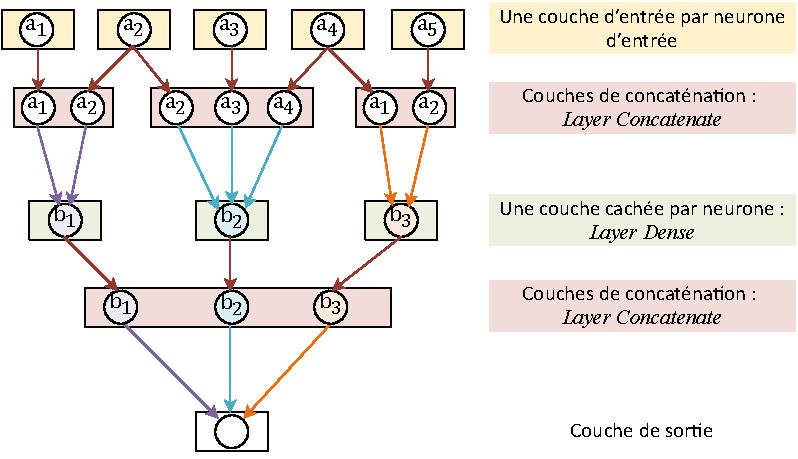
\includegraphics[height=8cm]{images_these/RN_dense_multiply.png}}
	\caption[Figure (\ref{RN_poids_fixes}) reformulé avec des layers Dense et Multiply.]{
		Figure (\ref{RN_poids_fixes}) reformulé avec des layers Dense et Multiply.}
	\label{RN_dense_multiply}
\end{figure}

L'extrait de code suivant montre comment programmer le réseau de la Figure (\ref{RN_dense_multiply}}).
\begin{lstlisting}
N = 8
M = 5

# création de 2 couches d'entrée de taille respective N et M
my_input1 = keras.Input(shape=(N,), name='input1') 
my_input2 = keras.Input(shape=(M,), name='input2') 

# une couche cachée 
couche1 = keras.layers.Dense(M, activation='linear', name='C1')(my_input1)

# multiplication de la couche d'entrée 'input2' et de la couche cachée
mult = keras.layers.Multiply()([my_input2, couche1])

# 1 neurone de sortie = somme des sorties de la couche précédente
# on a donc des fixes poids = 1 et un biais = 0
my_biais = np.asarray([0])
my_poids = np.ones((M,1))
sortie = keras.layers.Dense(1, activation='linear', name='out', weights=[my_poids, my_biais], trainable=False)(mult)

# création du modèle
model = keras.Model(inputs=[my_input1, my_input2], outputs=sortie)
\end{lstlisting}

%\section{Incertitudes}
\section{Conclusion}

Ce chapitre était consacré à l'établissement de l'état de l'art des methodes qu'on a exploré pour tenter de résoudre le problème traité dans le cadre de cette thèse. On a d'une part décrit ce qu'est la programmation dynamique et d'autre part décrit ce qu'est l'apprentissage. Le chapitre suivant sera consacré à la présentation de nos modèles.
%********************************************************************
\poubelle{
\section{Annexes}
\subsection{Démonstration du théorème \ref{dem_PTAS}}
\label{dem_PTAS_section}
Cette section présente la démonstration du théorème \ref{dem_PTAS}.
%\begin{proof}
Pour pouvoir réaliser cette démonstration, on va présenter l'algorithme $P^{\varepsilon}$. L'algorithme $P^{\varepsilon}$ procède comme suit : on calcule d'abord $K$ tel que $\varepsilon/2\leq 2^{-(K+N+1)}\leq \varepsilon$, puis on applique \textbf{PD-Knap}($K$). On choisit $K $tel que $2^{-(K+N +1)} \leq \varepsilon$ et on considère la suite d'état $e_1 = (0, 0), \dots, e^{Opt}_{N+1} = (a^{Opt}_{N+1}, w^{Opt}_{N+1})$ qui correspond au déroulé d'une solution associée à $V^{Opt}$. On vérifie alors par induction sur $i$ que, pour tout $i = 1,\dots, N+1$, on trouve, parmi les états de $E(i)$ générés selon \textbf{PD-Knap}($K$),  un état $(a_i, w_i)$ tel que : $a_i \leq a^{Opt}_i$  et  $w_i  \geq w^{Opt}_i \times (1- 2^{-( K+N +2-i)})$.
%\end{proof}
}